%
% Copyright (c) 2013-2023 Aleksey Fedoseev <aleksey@fedoseev.net>
% Copyright (c) 2015-2016 Alexander Shaenko <ark4110@gmail.com>
% Copyright (c) 2016-2023 Ilya Tagunov <tagunil@gmail.com>
% 
% Permission is granted to copy, distribute and/or modify this document
% under the terms of the GNU Free Documentation License, Version 1.3
% or any later version published by the Free Software Foundation;
% with no Invariant Sections, no Front-Cover Texts, and no Back-Cover Texts.
% A copy of the license is located here: http://www.gnu.org/copyleft/fdl.html.
%

\documentclass[12pt,a4paper]{article}
\usepackage[T2A]{fontenc}
\usepackage{ucs}
\usepackage[utf8]{inputenc}
\usepackage[english,russian]{babel}
\usepackage{indentfirst}
\usepackage{amsmath}
\usepackage{amssymb}
\usepackage{gensymb}
\usepackage{graphicx}
\usepackage{hyperref}
\usepackage{array}
\usepackage{titlesec}
\usepackage{subcaption}
\usepackage{wasysym}
\usepackage{longtable}
\usepackage{multirow}

\pagestyle{plain}
\parindent=1.25cm
\textheight=24cm
\textwidth=16cm
\topmargin=-1cm
\frenchspacing
\renewcommand{\theequation}{\thesection.\arabic{equation}}
\newcommand{\sectionbreak}{\clearpage}

\begin{document}

\title{%
  \textbf{Инженерный симулятор ОРБИТА 2.0} \\
    Руководство для преподавателя}

\author{
  Алексей Федосеев\\
  \texttt{aleksey@fedoseev.net}
  \and
  Александр Шаенко\\
  \texttt{ark4110@gmail.com}
  \and
  Илья Тагунов\\
  \texttt{tagunil@gmail.com}
}

\date{Версия 1.1, \today}

\maketitle

Этот текст распространяется под лицензией GNU Free Documentation License (FDL) версии
1.3. Подробную информацию об этой лицензии Вы можете на сайте GNU
\footnote{\url{http://www.gnu.org/copyleft/fdl.html}}.

Исходный текст находится в репозитории проекта на GitHub
\footnote{\url{https://github.com/dralex/orbita-simulator}}.

\tableofcontents

\clearpage
\section{Введение}

Симулятор «Орбита» позволяет спроектировать космический аппарат (КА), который должен
решить поставленную прикладную задачу на околоземной орбите. КА конструируется в виде
набора общих параметров и выбора подсистем, которые должны соответствовать общим
требованиям и решаемой задаче.

Симулятор позволяет рассчитать параметры КА в течение всего полёта и отображает переданную
на Землю телеметрию и результат полёта.

\subsection{Описание миссий}

Симулятор позволяет проходить следующие миссии:

\begin{description}
  \item[Тренировочная-1: Смотрим на Землю] КА стартует на орбите заданной
    высоты. Необходимо погасить начальное вращение аппарата и совершить полный оборот
    Земли с ориентацией аппарата в надир (нормально по отношению к поверхности). В этой
    тренировочной миссии аппарат будет полностью сконструирован, нужно будет только
    произвести расчёты и вставить в программу полёта нужные константы.
  \item[Тренировочная-2: Связь с Землёй] КА стартует на орбите заданной
    высоты. Необходимо запрограммировать аппарат для отправки сообщения на Землю через
    подсистему высокопроизводительной связи. В этой тренировочной миссии аппарат будет
    полностью сконструирован, нужно будет только написать его программу полёта.
  \item[Тренировочная-3: Орбитальный манёвр] КА стартует на орбите заданной
    высоты. Необходимо запрограммировать аппарат для перехода на более высокую орбиту. В
    этой тренировочной миссии аппарат будет полностью сконструирован, нужно будет только
    рассчитать необходимую массу топлива и написать программу полёта.
  \item[Дистанционное зондирование Земли] КА стартует на орбите заданной высоты. Вам
    необходимо сделать из космоса снимок объекта расположенного на Земле. Данные снимка
    нужно передать в наземный измерительный пункт (НИП) по высокопроизводительному каналу
    связи. Количество полученных победных очков зависит от разрешения снимка и
    нормальности ориентации аппарата по отношению к поверхности в момент съёмки.
  \item[SMS везде] КА стартует на орбите заданной высоты. Команде выдаётся набор
    сообщений, которые должны быть доставлены между НИП-ами. Необходимо последовательно
    переориентировать аппарат на НИП-ы, чтобы принять сигнал от одних станций и передать
    его на другие. Количество полученных победных очков зависит от числа переданных на
    Землю сообщений.
  \item[Инспекция спутника] КА стартует на орбите заданной высоты. Известна другая орбита,
    по которой движется спутник-цель. Необходимо приблизиться к цели, чтобы
    сфотографировать его и передать результаты съёмки на Землю. Количество полученных
    победных очков зависит от разрешения снимка.
  \item[Белковый кристалл в невесомости] КА стартует на орбите заданной высоты. Ваша
    задача – вырастить в невесомости белковый кристалл и доставить его на Землю. Для этого
    Вам нужно вывести спутник на заданную орбиту, сделать один оборот вокруг планеты с
    выключенной аппаратурой (включёнными могут быть только бортовая вычислительная
    система, подсистема электропитания и сам контейнер с кристаллом), сохраняя температуру
    КА в требуемом диапазоне, а затем посадить аппарат в определённую точке земной
    поверхности. Количество полученных победных очков зависит от точности посадки.
  \item[Спутник связи <<Молния>>] Миссия моделирует ситуацию, в которой необходимо, имея
    ограниченный ресурс по топливу и параметрам КА, организовать несколько сеансов
    продолжительной радиосвязи с наземным измерительным пунктом. Оказывается, что
    привычные круговые орбиты для решения задачи не подходят и участникам нужно будет
    придумать, чем их заменить.
  \item[Система предупреждения о ракетном нападении] КА находится на геостационарной
    орбите, выполняя функцию предупреждения запусков ракет. Во время разгона
    баллистическая ракета выделяет большое количество энергии и хорошо заметна в
    инфракрасном диапазоне. Находящийся на орбите КА с помощью инфракрасной камеры может
    легко идентифицировать место старта ракеты и отправляет координаты запуска на Землю,
    что делает возможным перехват.
\end{description}

В данном руководстве мы опишем принципы конструирования КА, а также все используемые в
симуляторе математические модели. Вы также сможете познакомиться с подробным описанием и
условиями миссий в разделе \ref{Sec:Missions}.

\section{Конструирование аппарата}

КА представляется в виде систем-блоков, описываемых набором параметров и объединённых
различного рода связями. Для моделирования доступны следующие десять блоков (подсистем),
семь из которых являются обязательными для любого КА (см. рисунок \ref{Pic:subsystems}).

\begin{figure}[tbh]
  \begin{center}
    \includegraphics[width=12cm]{images/subsystems-ru.eps}
    \caption{Схема подсистем КА}
    \label{Pic:subsystems}
  \end{center}
\end{figure}

Каждая из подсистем характеризуется следующим набором параметров:

\begin{itemize}
\item масса (кг);
\item объем (л);
\item допустимый температурный режим: мин./макс. (°С);
\item энергопотребление (Вт);
\item тепловыделение (Вт);
\item текущее состояние (вкл., выкл., неисправно).
\end{itemize}

Рассмотрим подробнее назначение каждой из подсистем и их специальные параметры
(\textbf{*}~--- обязательная подсистема):

\begin{description}
\item[Конструктив (корпус) аппарата (*)] Корпус составляет внешний контур КА, а также
  используется для монтажа всех систем КА. К специальным параметрам конструктива
  относится:
  \begin{itemize}
    \item размер стороны куба, м.
  \end{itemize}
\item[Бортовая вычислительная система (*)] БВС содержит основную программу полёта и набор
  служебных параметров. К специальным параметрам БВС относится:
  \begin{itemize}
    \item оперативная память, МБ.
  \end{itemize}
\item [Система электропитания (*)] Система электропитания (СЭ) обеспечивает электрической энергией
  все системы КА. Как правило эта система состоит из аккумулятора и набора солнечных
  батарей, а также системы управления питанием. К специальным параметрам СЭ относятся:
  \begin{itemize}
  \item ёмкость аккумулятора, $\text{Вт} - \text{ч}$;
  \item КПД солнечных батарей, \%;
  \item коэффициент поглощения тепла солнечными батареями;
  \item коэффициент черноты солнечных батарей.
  \end{itemize}

\item [Система навигации (*)] Система навигации содержит специальный вычислитель и набор
  датчиков, позволяющих с высокой точностью определить положение аппарата относительно
  Земли. Не имеет специальных параметров.

\item [Система управления ориентацией и стабилизацией (*)] Система управления ориентации и
  стабилизацией (СУОС) обеспечивает ориентацию аппарата в заданном направлении. К
  специальным параметрам СУОС относится:
  \begin{itemize}
    \item максимальный момент, $\text{Н} \cdot \text{м}$.
  \end{itemize}

\item [Система обеспечения теплового режима (*)] Система обеспечения теплового
  режима (СОТР) служит для поддержания требуемого температурного режима аппарата. Как правило,
  эта система содержит датчики температуры, нагреватели и радиатор, который может излучать
  излишки тепла в космическое пространство. К специальным параметрам СОТР относятся:
  \begin{itemize}
  \item коэффициент поглощения тепла радиаторами;
  \item коэффициент черноты радиатора;
  \item мощность нагревателя, Вт.
  \end{itemize}

\item [Система телеметрии (*)] Система телеметрии предназначена для передачи на Землю
  служебных сообщений о состоянии аппарата и его систем. Как правило, эта система содержит
  независимый передатчик малой мощности. К специальным параметрам системы телеметрии
  относятся:
  \begin{itemize}
  \item усиление бортовой антенны;
  \item усиление наземной антенны;
  \item угол раскрыва антенны, °;
  \item мощность передатчика, Вт.;
  \item частота (МГц)
  \end{itemize}
  
\item [Система высокопроизводительной связи] Система высокопроизводительной связи
  позволяет передавать на Землю данные большого объёма за короткие периоды
  времени. Система высокопроизводительной связи имеет те же специальные параметры, что и
  система телеметрии (см. выше).

\item [Система изменения орбиты] Система изменения орбиты содержит двигательную установку
  и топливные баки.
  \begin{itemize}
    \item максимальный массовый расход топлива, кг/с;
    \item удельный импульс двигательной установки, м/с;
    \item объем топливных баков, л.
  \end{itemize}

\item [Полезная нагрузка (вариант 1~--- камера)] Камера позволяет производить цифровые
  снимки объектов на Земле и в космосе. К специальным параметрам камеры относятся:
  \begin{itemize}
  \item угол поля зрения, °;
  \item спектральный диапазон;
  \item поток данных, Мбит/с;
  \item объем памяти, МБ;
  \item матрица, пикс.
  \end{itemize}

\item [Полезная нагрузка (вариант 2~--- контейнер для кристалла)] Контейнер предназначен
  для выращивания белковых кристаллов и последующей их транспортировки на Землю. Контейнер
  содержит жаропрочные стенки, парашют и систему амортизации при посадке на
  Землю. Контейнер не имеет специальных параметров.

\end{description}

Полный список подсистем, доступных для конструирования, представлен в Приложении 1.

Корпус аппарата для простоты моделирования принимается за имеющий кубическую форму,
доступны корпуса разного размера. Таким образом, аппарат имеет шесть внешних поверхностей
(см. рисунок \ref{Pic:cube}).

\begin{figure}[tbh]
  \begin{center}
    \includegraphics[width=6cm]{images/cube.eps}
    \caption{Принципиальная пространственная модель КА}
    \label{Pic:cube}
  \end{center}
\end{figure}

Нумерация поверхностей с 1 по 4 идёт против часовой стрелки, поверхности 5 и 6 находятся в
плоскости X0Y, при этом поверхность 5 имеет большую координату по оси Z. С учетом того,
что в данной модели аппарат движется в плоскости X-Y, грани 5 и 6 всегда параллельны
плоскости движения аппарата.

Компоновка подсистема внутри аппарата в модели не рассматривается, однако некоторые
подсистемы имеют выводы на поверхности корпуса:

\begin{itemize}
\item антенна системы высокопроизводительной связи и полезная нагрузка (камера)
  расположены на поверхности 1;
\item поверхности 1-4 могут содержать элементы солнечных батарей и радиаторов; при
  конструировании указывается соотношение площадей солнечных батарей, радиаторов и
  незанятой поверхности~--– одинаковое для всех четырёх поверхностей;
\item поверхности 5-6 в данной модели никогда не освещаются Солнцем, поэтому для них можно
  указать соотношение площадей радиаторов и незанятой поверхности~--– одинаковое для обеих
  поверхностей.
\end{itemize}

Также аппарату можно задать массу заливаемого топлива (кг). Топливо заданной массы должно
вмещаться в топливные баки, установленные на КА (объем баков определён в параметрах
системы изменения орбиты). Вне зависимости от выбора используемого двигателя, применяется
единственный тип топлива: \textbf{АТ+НДМГ}, плотность которого равна \textbf{1185
  $\text{кг}/\text{м}^3$}.

При конструировании КА следует учитывать также следующее ограничение: максимальная масса
КА не должна превышать \textbf{20 тонн}.

\section{Моделирование космического аппарата}

Моделирование полёта КА происходит с задаваемым или автоматически выбираемым шагом по
времени. На каждом шаге во времени проводится анализ взаимодействия блоков. На данном
этапе симулятор производит следующие расчёты:

\begin{enumerate}
  \item баллистический расчёт (расчёт положения центра масс КА);
  \item механический расчёт (расчёт нагрузок, действующих на КА, и изменение ориентации КА под их действием);
  \item энергетический расчёт;
  \item тепловой расчёт;
  \item расчёт информационного обмена;
  \item выполнение программ полета;
  \item работа полезной нагрузки.
\end{enumerate}

\subsection{Баллистический расчёт}
\label{Sec:Ballistics}

В модели принято, что КА совершает полёт вокруг Земли в центральном поле
тяготения. Положение КА описывается в системе координат, начало отсчёта которой находится
в центре масс Земли, оси $x$ и $y$ располагаются в плоскости орбиты, ось $z$ пополняется систему
до правой тройки векторов. Система координат показана на рисунке \ref{Pic:Coord}. КА
совершает полёт в плоскости орбиты $X0Y$.

\begin{figure}[tbh]
  \begin{center}
    \includegraphics[width=12cm]{images/coord-ru.eps}
    \caption{Система координат в баллистическом и механическом расчётах}
    \label{Pic:Coord}
  \end{center}
\end{figure}

Положение КА измеряется системой навигации без погрешности.

В начальный момент времени КА имеет координаты, равные $(0, h_{\text{орб}} + R_{\text{З}},
0)$, где $h_{\text{орб}}$~--– высота начальной орбиты аппарата, а $R_{\text{З}}$~--–
радиус Земли. В любой момент времени положение аппарата задаётся координатами
$(X_{\text{КА}}, Y_{\text{КА}}, 0)$ или парой из угла положения аппарата $\alpha$
(начальное значение равно 0, увеличивается по часовой стрелке от оси $y$) и текущей высоты орбиты
$h_{\text{орб}}$. Также аппарат характеризуется углом ориентации $\varphi$ (начальное значение
которого равно 0, увеличивается против часовой стрелки от оси $x$). \textbf{Все расстояния в модели
измеряются в метрах (если не сказано иначе), углы~--- в градусах.}

Положение Солнца в данной модели постоянно и равно $(+\infty, 0, 0)$. Соответственно, освещённой
оказывается одна и та же половина Земли.

На КА в полёте действуют следующие три силы:

\begin{itemize}
\item сила гравитационного притяжения к Земле;
\item сила тяги двигателя (если двигатель установлен на КА и включен);
\item сила аэродинамического сопротивления (если аппарат достиг земной атмосферы).
\end{itemize}

Все силы также действуют только в плоскости орбиты $X0Y$.

\paragraph{Сила гравитационного притяжения}

В произвольный момент времени космический аппарат находится в точке с координатами $(X_{\text{КА}},
Y_{\text{КА}}, 0)$, при этом на него действует сила гравитационного притяжения к Земле $F_{\text{Г}}$,
см. рисунок \ref{Pic:Gravity}.

\begin{figure}[tbh]
  \begin{center}
    \includegraphics[width=10cm]{images/gravity-ru.eps}
    \caption{Положение КА на орбите и направление силы гравитационного притяжения к Земле}
    \label{Pic:Gravity}
  \end{center}
\end{figure}

Величина силы вычисляется согласно закону всемирного тяготения \ref{Eq:gravity}:

\begin{eqnarray}
  F_{\text{Г}} = G \frac{m_{\text{КА}} M_{\text{З}}}{R_{\text{КА}}^2}, \label{Eq:gravity}
\end{eqnarray}

где $G$~--- гравитационная постоянная, равная $6,67384 \cdot 10^{-11} \text{м}^3
\text{кг}^{-1} \text{с}^{-2}$; $m_{\text{КА}}$~--- текущая масса КА, кг; $M_{\text{З}}$~--–
масса Земли, равная $5,97 \cdot 10^{24} \text{кг}$; $R_{\text{КА}}$~--– длина радиус-вектора
КА в текущий момент времени.

Величина скорости аппарата при движении по орбите вычисляется по формуле:

\begin{eqnarray}
  v_{\text{орб}} = \sqrt{\frac{G M_{\text{З}}}{R_{\text{З}} + h_{\text{орб}}}}, \label{Eq:orbital-velocity}
\end{eqnarray}

где $G$~--- гравитационная постоянная, а $M_{\text{З}}$~--- масса Земли.

Длину радиус-вектора КА в текущий момент времени RКА можно вычислить по формуле
\ref{Eq:radius-vector}:

\begin{eqnarray}
  R_{\text{КА}} = \sqrt{X_{\text{КА}}^2 + Y_{\text{КА}}^2}, \label{Eq:radius-vector}
\end{eqnarray}

Проекции силы гравитационного притяжения $F_{\text{Г}}$, обозначенной на рисунке
\ref{Pic:Gravity} на оси системы координат можно записать в следующем виде
(\ref{Eq:gravity-force}):

\begin{eqnarray}
  F_{\text{Г}}^X = - G \frac{m_{\text{КА}} M_{\text{З}}}{\left(X_{\text{КА}}^2 +
    Y_{\text{КА}}^2\right)^{\frac{3}{2}}} X_{\text{КА}}, \nonumber \\
  F_{\text{Г}}^Y = - G \frac{m_{\text{КА}} M_{\text{З}}}{\left(X_{\text{КА}}^2 +
    Y_{\text{КА}}^2\right)^{\frac{3}{2}}} Y_{\text{КА}} \label{Eq:gravity-force}
\end{eqnarray}

\paragraph{Сила тяги двигателя} 

С корпусом КА связана также система координат, начало отсчёта которой располагается в
центре масс аппарата. В начальный момент времени оси системы координат располагаются
параллельно осям системы координат Земли, показанной на рисунке \ref{Pic:Coord}. При
отсутствии вращения КА относительно собственного центра масс оси систем координат остаются
параллельными в процессе всего витка, см. рисунок \ref{Pic:Coord-Sat}.

\begin{figure}[tbh]
  \begin{center}
    \includegraphics[width=10cm]{images/coord-sat-ru.eps}
    \caption{Взаимное расположение систем координат Земли и КА}
    \label{Pic:Coord-Sat}
  \end{center}
\end{figure}

Ориентация КА задаётся углом поворота $\varphi$ (или $\varphi_Z$) оси $X_{\text{КА}}$ относительно оси $X$ системы координат
Земли, что соответствует вращению КА относительно оси $Z$. Угол поворота задаёт направление
плоскости аппарата.

Направление силы тяги двигателя жёстко связано с направлением оси $x_{\text{КА}}$ системы
координат КА, что приводит к необходимости изменять ориентацию КА для изменения
направления силы тяги. Состояние системы коррекции орбиты (СКО) контролируется системой
управления. Величина тяги регулируется дискретно: либо СКО включена и создаёт тягу, либо
СКО выключена и тяги не создаёт.

Величина тяги при включённой двигательной установке вычисляется по формуле
\ref{Eq:traction-force}:

\begin{eqnarray}
  F_{\text{Т}} = \Delta m I_{\text{уд}}, \label{Eq:traction-force}
\end{eqnarray}

где $\Delta m$~--– массовый расход компонент топлива, кг/с, $I_{\text{уд}}$~---– удельный
импульс двигательной установки, м/с.

Очевидно, что двигательная установка может создавать тягу в том случае, когда в баках
системы изменения орбиты ещё осталось топливо. Зависимость массы топлива $m_{\text{Т}}$ от времени
работы двигательной установки $t_{\text{ДУ}}$ при включённой системе изменения обриты выглядит
следующим образом:

\begin{eqnarray}
  m_{\text{Т}} = m_{\text{Т}}^0, - \Delta m t_{\text{ДУ}}
\end{eqnarray}

где $m_{\text{Т}}^0$~--– масса топлива в баках системы изменения орбиты перед включением,
кг.

Проекции силы тяги на оси системы координат Земли можно записать в следующем виде
(\ref{Eq:traction-force-proj}):

\begin{eqnarray}
  F_{\text{Т}}^X = \Delta m I_{\text{уд}} \cos{\varphi_Z} \nonumber \\
  F_{\text{Т}}^Y = \Delta m I_{\text{уд}} \sin{\varphi_Z} \label{Eq:traction-force-proj}
\end{eqnarray}

\paragraph{Сила аэродинамического сопротивления}

Сила аэродинамического сопротивления FА возникает при движении КА в верхних слоях
атмосферы, величина силы рассчитывается по формуле \ref{Eq:stokes}:

\begin{eqnarray}
  F_{\text{А}} = C_\xi \frac{\rho V_{\text{КА}}^2}{2} S_{\text{КА}}, \label{Eq:stokes}
\end{eqnarray}

где $C_\xi$~--– коэффициент аэродинамического сопротивления КА, равный $1,05$ (значение
для куба); $\rho$~--– плотность атмосферы на текущей высоте полёта КА\footnote{См. ГОСТ
  4401-81~--— Атмосфера стандартная. Параметры, например в Википедии},
$\text{кг}/\text{м}^3$; $V_{\text{КА}}$~--– текущая скорость полёта КА, м/с;
$S_{\text{КА}}$~--– площадь поперечного сечения КА, $\text{м}^2$. Сила аэродинамического
сопротивления $F_{\text{А}}$ направлена противоположно вектору скорости КА, см. рисунок
\ref{Pic:Stokes}.

\begin{figure}[tbh]
  \begin{center}
    \includegraphics[width=10cm]{images/stokes-ru.eps}
    \caption{Направление силы аэродинамического сопротивления $F_{\text{А}}$ и её проекций
      на оси системы координат, связанной с Землёй}
    \label{Pic:Stokes}
  \end{center}
\end{figure}

Для вычисления проекций силы аэродинамического сопротивления на оси системы координат, связанной с
Землёй, $F_{\text{А}}^X$ и $F_{\text{А}}^Y$ воспользуемся разложением скорости на проекции
(формула \ref{Eq:velocity-vector}).

\begin{eqnarray}
  V_{\text{КА}}^2 = \left( V_{\text{КА}}^X \right)^2 + \left( V_{\text{КА}}^Y \right)^2
  \label{Eq:velocity-vector}
\end{eqnarray}

и тогда проекции, соответствующие рисунку \ref{Pic:Stokes}, вычисляются по формулам
\ref{Eq:stokes-proj}:

\begin{eqnarray}
  F_{\text{A}}^X = - C_\xi \frac{\rho \left| V_{\text{КА}}^X \right| V_{\text{КА}}^X}{2} S_{\text{КА}} \nonumber \\
  F_{\text{A}}^Y = - C_\xi \frac{\rho \left| V_{\text{КА}}^Y \right| V_{\text{КА}}^Y}{2} S_{\text{КА}} \label{Eq:stokes-proj}
\end{eqnarray}

\paragraph{Интегрирование уравнений движения центра масс КА}

Полный набор уравнений движения получается подстановкой уравнений для проекций сил
\ref{Eq:gravity}, \ref{Eq:traction-force} и \ref{Eq:stokes} в уравнение второго закона
Ньютона, записанное для двух проекций на оси системы координат, связанной с Землёй:

\begin{eqnarray}
  m_{\text{КА}} \cdot a_{\text{КА}}^X = F_{\text{Г}}^X + F_{\text{Т}}^X + F_{\text{А}}^X
  \nonumber \\
  m_{\text{КА}} \cdot a_{\text{КА}}^Y = F_{\text{Г}}^Y + F_{\text{Т}}^Y + F_{\text{А}}^Y
\end{eqnarray}

Движение центра масс КА может быть промоделировано с помощью специального баллистического
калькулятора (см. раздел \ref{Sec:Calculator}).

\subsection{Механический расчёт}
\label{Sec:Mechanics}

В начальный момент времени $t_0 = 0$ космический аппарат имеет угловую скорость $\omega_0
= 1\degree/\text{с}$ относительно оси $Z$. Угловая скорость аппарата меняется по формуле:

\begin{eqnarray}
  \omega(t) = \omega_0 + \varepsilon t,
\end{eqnarray}

где $\varepsilon$~--- угловое ускорение аппарата, $\degree/\text{с}^2$.

Угловая скорость и угол ориентации КА измеряется системой ориентации без
погрешности. Изменение угла ориентации аппарата определяется по формуле:

\begin{eqnarray}
  \varphi(t) = \varphi_0 + \omega t + \frac{\varepsilon t^2}{2},
\end{eqnarray}

где $\varphi_0$~--- стартовая ориентация аппарата.

Изменение ориентации КА производится с помощью двигателя-маховика или другого
устройства\footnote{В текущей версии руководства рассматривается только модель маховика.},
входящего в состав системы управления ориентацией и стабилизацией (СУОС). Считается, что
маховик не имеет предельной скорости вращения, поэтому нет необходимости проводить
операцию сброса накопившегося кинетического момента.

С учётом описанных допущений уравнение, описывающее вращательную динамику КА, можно
записать в виде (формула \ref{Eq:flywheel}):

\begin{eqnarray}
  I_z \varepsilon = M_Z(t) \label{Eq:flywheel}\\
  \varepsilon = \frac{M_Z}{I_Z}, \label{Eq:angular-acceleration}
\end{eqnarray}

где $I_Z$~--- момент инерции КА при вращении относительно оси $Z$, $\text{кг} \cdot \text{м}^2$;
$M_Z(t)$~--- момент, создаваемый двигателем-маховиком относительно оси $Z$, $\text{Н}
\cdot \text{м}$. Момент может задаваться программой полёта в допустимых для данного
двигателя-маховика предела.

В данной модели КА представляет собой куб заданного размера. Мы считаем, что масса
аппарата распределена равномерно по его объему, поэтому момент инерции аппарата считается
следующим образом:

\begin{eqnarray}
  I_z = \frac{1}{12} (2 a^2) m(t), \label{Eq:inertia-moment}
\end{eqnarray}

где $a$~--– размер грани аппарата, м; $m(t)$~--- масса аппарата в момент времени $t$.

Вращение КА аппарата вокруг центра масс может быть промоделировано с помощью специального
механического калькулятора (см. раздел \ref{Sec:Calculator}).

\subsection{Энергетический расчёт}
\label{Sec:Energy}

В каждый момент времени аппарат характеризуется потребляемой $P_{\text{потр}}$ и
вырабатываемой $P_{\text{выраб}}$ мощностью. Потребляемая мощность складывается из
потребления всех включённых устройств (которые находятся в состоянии \verb'ON'):

\begin{eqnarray}
  P_{\text{потр}} = \sum_i{P_{i}^{ON}}
\end{eqnarray}

Вырабатываемая мощность складывается из тока, вырабатываемого солнечными батареями~--–
фотоэлектрическими элементами~--- и тока, поступающего от аккумуляторной батареи.

\begin{eqnarray}
  P_{\text{выраб}} = P_{\text{ФЭП}} + P_{\text{аккум}}
\end{eqnarray}

Фотоэлектрические элементы (ФЭП) расположены на боковых гранях аппарата (1-4). Считается,
что солнце освещает одну из граней. Электрическая мощность, вырабатываемая ФЭП,
вычисляется следующим образом (формула \ref{Eq:photoelement}):

\begin{eqnarray}
  P_{\text{ФЭП}} = \eta_{\text{ФЭП}} \cdot S_{\text{ФЭП}} \cdot q_{\text{С}}(t), \label{Eq:photoelement}
\end{eqnarray}

где $\eta_{\text{ФЭП}}$~--- КПД ФЭП; $S_{\text{ФЭП}}$~--- суммарная площадь ФЭП на
освещённой грани аппарата, $\text{м}^2$; $q_{\text{С}}(t)$~--– плотность потока солнечного
излучения, $\text{Вт} \cdot \text{м}^{-2}$, которая определяется в зависимости от положения
космического аппарата на орбите (см. рисунок \ref{Pic:Coord}) по формуле \ref{Eq:sunlight}:

\begin{eqnarray}
  q_{\text{С}}(t) = \left\{
  \begin{array}{l}
    0, \text{при}~X_{\text{КА}}(t) < 0~\text{и}~|Y_{\text{КА}}(t)| \leqslant R_{\text{З}}\\
    1400, \text{во всех других случаях.}
  \end{array}
\right. \label{Eq:sunlight} 
\end{eqnarray}

Считается, что при любой ориентации аппарата Солнце будет освещать площадь, равную площади
солнечных батарей, расположенных на боковой поверхности корпуса (1-4). Площадь ФЭП
определяется по формуле:

\begin{eqnarray}
  S_{\text{ФЭП}} = k^{(1-4)}_{\text{сб}} \cdot a^2, \label{Eq:photopanels}
\end{eqnarray}

где $k^{(1-4)}_{\text{сб}}$~--- доля солнечных батарей на каждой из поверхностей 1-4
аппарата (параметр конструирования), $a$~--– длина грани аппарата, м.

Бортовая химическая аккумуляторная батарея характеризуется ёмкостью, $\text{Вт}-\text{ч}$. Возможны
следующие варианты:

$$
 \left\{
  \begin{array}{l}
    P_{\text{потр}} < P_{\text{выраб}}, \text{излишки электроэнергии заряжают
      аккумулятор};\\
    P_{\text{потр}} = P_{\text{выраб}}, \text{аккумулятор не используется};\\
    P_{\text{потр}} > P_{\text{выраб}}, \text{тока солнечных батарей не достаточно,
      используется аккумулятор}.\\
  \end{array}
\right.
$$

Аккумуляторная батарея компенсирует потребление аппарата, если вырабатываемого солнечными
батареями тока не достаточно для работы. Если же вырабатываемый ток превышает
потребляемый, батарея может подзаряжаться. Излишки электроэнергии, не пошедшие на зарядку
аккумулятора, сбрасываются на резистор, т.е. игнорируются.

\paragraph{Нехватка электроэнергии}

Отдельного рассмотрения требует случай нехватки электроэнергии. Если подсистемы аппарата
потребляют энергии больше, чем подсистема электропитания может выдавать, аппарат переходит
в режим экономии питания (\verb'SAFE MODE'), в котором остаются включёнными только три
подсистемы: сама система электропитания, бортовая вычислительная система и подсистема
телеметрии, остальные подсистемы выключаются. В этом случае бортовая вычислительная
система переходит в режим \verb'STATE_SAFE'. Переход в нормальный режим работы аппарата
осуществляется через изменение режима работы бортовой вычислительной системы на
\verb'STATE_WAKEUP' (см. раздел \ref{Sec:CPU}). В случае нехватки электроэнергии уже в режиме экономии
питания, аппарат выходит из строя.

\subsection{Тепловой расчёт}
\label{Sec:Heat}

Мы принимаем, что в моделируемом КА отдельные блоки аппаратуры соединены тепловыми связями
с малым термическим сопротивлением, что приводит к выравниваю поля температуры по всем
космическому аппарату. Другими словами, температура КА характеризуется единственной
величиной~--– $T$, К.

Температура КА $T$ влияет на работу устройств. Каждая подсистема обладает двумя
характеристиками: минимальной и максимальной допустимой температурой. При пересечении
любой из двух границ подсистема выходит из строя (\emph{обратите внимание, что температурный
режим подсистем задан в градусах Цельсия, а данная модель и телеметрия аппарата оперирует
Кельвинами}).

Температура КА $T$ меняется от времени следующим образом (формула \ref{Eq:temperature}):

\begin{eqnarray}
c \cdot m(t) \cdot \frac{\Delta T}{\Delta t} = Q^{\Sigma}_{\text{внешн}} + Q^{\Sigma}_{\text{внутр}}, \label{Eq:temperature}
\end{eqnarray}

где $c$~--- средняя удельная теплоёмкость материалов КА, равная \textbf{800 $\text{Дж}
  \cdot \text{кг}^{-1} \cdot \text{К}^{-1}$}; $m(t)$~--– масса КА в момент времени $t$;
$Q^{\Sigma}_{\text{внешн}}$~--- слагаемое, описывающее внешний теплообмен КА;
$Q^{\Sigma}_{\text{внутр}}$~--– сумма тепловыделений подсистем бортовой аппаратуры в
момент времени $t$.

Внешний теплообмен считается для всей поверхности аппарата как показано на рисунке \ref{Pic:heat-exchange}.

\begin{figure}[tbh]
  \begin{center}
    \includegraphics[width=7cm]{images/heat-exchange.eps}
    \caption{Внешний теплообмен КА}
    \label{Pic:heat-exchange}
  \end{center}
\end{figure}

Считается, что одна грань аппарата (одна из поверхностей 1-4), наиболее близкая к Солнцу,
нагревается тепловым потоком. При конструировании аппарата указывается соотношение
площадей солнечных батарей, радиатора и теплоизолятора, поскольку они нагреваются
по-разному: коэффициент поглощения тепла для солнечных батарей и радиатора указывается в
параметрах подсистем, а для теплоизолятора он равен 0.

Одновременно с этим, все грани аппарата излучают тепло. Солнечные батареи и радиаторы
имеют разную степень черноты, указанную в параметрах подсистем, а чернота теплоизолятора
считается равной 0.

Таким образом, внешний теплообмен КА вычисляется по формуле \ref{Eq:heat-exchange}:

\begin{eqnarray}
  Q^{\Sigma}_{\text{внешн}} = \left(S_{\text{сб}}^{\text{погл}} A_{\text{сб}} +
  S_{\text{рад}}^{\text{погл}} A_{\text{рад}}\right) \cdot q_{\text{С}}(t) -
  \left(S_{\text{сб}}^{\text{изл}} \varepsilon_{\text{сб}} + S_{\text{рад}}^{\text{изл}}
  \varepsilon_{\text{рад}}\right)
  \sigma T^4, \label{Eq:heat-exchange}
\end{eqnarray}

где $S_{\text{сб}}^{\text{погл}}$~--- площадь поглощения тепла солнечными батареями,
$\text{м}^2$; $A_{\text{сб}}$~--– коэффициент поглощения солнечного излучения солнечными
батареями; $S_{\text{сб}}^{\text{погл}}$~--– площадь поглощения тепла от солнца
радиаторами, $\text{м}^2$; $A_{\text{сб}}$~--– коэффициент поглощения солнечного излучения
радиаторами; $q_{\text{С}}(t)$~--– плотность потока солнечного излучения, $\text{Вт} \cdot
\text{м}^{-2}$, которая была определена ранее в \ref{Eq:sunlight};
$S_{\text{сб}}^{\text{изл}}$~--- площадь излучения солнечными батареями КА, $\text{м}^2$; $\varepsilon_{\text{сб}}$~--–
степень черноты солнечных батарей; $S_{\text{рад}}^{\text{изл}}$~--– площадь излучения
всеми радиаторами КА, $\text{м}^2$; $\varepsilon_{\text{рад}}$~--– степень черноты радиатора; $\sigma$~--- постоянная в законе
Стефана-Больцмана, равная $5,67 \cdot 10^{-8} \cdot \text{Дж} \cdot \text{с}^{-1} \cdot
\text{м}^{-2} \cdot \text{К}^{-4}$.

\begin{figure}[tbh]
  \begin{center}
    \includegraphics[width=15cm]{images/surfaces.eps}
    \caption{Расположение солнечных батарей и радиаторов на гранях аппарата}
    \label{Pic:surfaces}
  \end{center}
\end{figure}

Необходимые площади вычисляются следующим образом:

\begin{eqnarray}
  \begin{array}{l}
  S_{\text{сб}}^{\text{погл}} = k^{(1-4)}_{\text{сб}} \cdot a^2 \\
  S_{\text{рад}}^{\text{погл}} = k^{(1-4)}_{\text{рад}} \cdot a^2 \\
  S_{\text{сб}}^{\text{изл}} = 4 \cdot k^{(1-4)}_{\text{сб}} \cdot a^2 \\
  S_{\text{рад}}^{\text{изл}} = (4 \cdot k^{(1-4)}_{\text{рад}} + 2 \cdot
  k^{(5-6)}_{\text{рад}}) \cdot a^2
  \end{array}
\end{eqnarray}

где $a$~--- размер ребра аппарата, м; $k^{(1-4)}_{\text{сб}}$~--- доля площади солнечных батарей на каждой из
поверхностей 1-4; $k^{(1-4)}_{\text{рад}}$~--- доля площади радиаторов на каждой из поверхностей 1-4;
$k^{(5-6)}_{\text{рад}}$~--- доля площади радиаторов на каждой из поверхностей 5-6.

При конструировании аппарата необходимо указать долю солнечных батарей и радиаторов на
гранях 1-4 и долю радиаторов на гранях 5-6. Остальная поверхность покрывается специальной
плёнкой, которая препятствует теплообмену (см. рисунок \ref{Pic:surfaces}).

Массой солнечных батарей и радиаторов можно пренебречь.

Сумма тепловыделений подсистем КА вычисляется только для включённых подсистем по формуле
\ref{Eq:heat_prod}:

\begin{eqnarray}
Q^{\Sigma}_{\text{внутр}}(t) = \sum_i Q_{i}^{ON}(t), \label{Eq:heat_prod}.
\end{eqnarray}

Подсистема СОТР аппарата имеет дополнительные нагреватели, которые можно включать в
программе полёта. Таким образом, аппарат можно дополнительно подогревать изнутри, если это
будет необходимо.

\subsection{Расчёт информационного обмена}
\label{Sec:Radio}

КА вступает в информационный обмен с одним или несколькими наземными комплексами
управления посредством радиосвязи. Примем, что связь между КА и Землёй устроена одинаково
в обоих направлениях (от КА к наземным измерительным пунктам (НИП) или
наоборот). Координаты НИП заданы в условиях решения задачи. Будем считать, что антенна НИП
постоянно отслеживает траекторию КА.

Бортовая антенна аппарата закреплена неподвижно на корпусе аппарата (на поверхности 1) и
имеет диаграмму направленности с углом раскрыва, заданным в параметрах передающей
антенны. Диаграмма направленности бортовой антенны располагается так, что делится пополам
вектором ориентации КА (см. рисунок \ref{Pic:Radio}). Существуют антенны с углом раскрыва, равным 360°.

Сигнал антенны экранируется Землёй.

\begin{figure}[tbh]
  \begin{center}
    \includegraphics[width=12cm]{images/radio.eps}
    \caption{Направленность антенны КА}
    \label{Pic:Radio}
  \end{center}
\end{figure}

Мощность сигнала $P_2$ на входе в приёмник НИП рассчитывается по формуле
\ref{Eq:gs-signal}:

\begin{eqnarray}
P_2 = \frac{G_1 G_2 \Delta_2 P_1}{b_1 b_2 L_{12}}, \label{Eq:gs-signal}.
\end{eqnarray}

где $P_1$~--– мощность передатчика КА, Вт; $G_1$ и $G_2$~--– усиления бортовой и наземной
антенн, которые зависят от типа антенны и заданы в параметрах подсистем; $b_1$ и $b_2$~--–
потери в бортовом и наземном радиотракте (считаем, что $b_1 = 1$ и $b_2 = 1$);
$\Delta_2$~--– потери за счёт неточного наведения приёмной антенны на КА (считаем, что
потери отсутствуют и $\Delta_2 = 1$); $L_{12}$~--– ослабление сигнала на пути от КА до
НИП, рассчитываемое по формуле \ref{Eq:signal-attenuation}:

\begin{eqnarray}
L_{12} = \left( \frac{4 \pi L_{\text{НИП}}}{\lambda_1} \right)^2 \Delta L_{12}, \label{Eq:signal-attenuation}.
\end{eqnarray}

где $L_{\text{НИП}} = \sqrt{(X_{\text{НИП}} - X_{\text{КА}})^2 + (Y_{\text{НИП}} -
  Y_{\text{КА}})^2 + (Z_{\text{НИП}} - Z_{\text{КА}})^2}$~--- расстояние КА до НИП, м
(напомним, что в данной модели координата $Z = 0$); $\lambda_1$~--- длина волны передатчика
(считается через частоту передачи, заданную в параметрах подсистемы); $\Delta L_{12}$~---
потери за счёт неидеальности среды (считаем, что потери отсутствуют и $\Delta L_{12} = 1$). Если НИП
не находится в створе диаграммы направленности передающей антенны, $G_1 = 0$.

В радиоканале используется фазовая модуляция с четырехкратной манипуляцией. Мощность шумов
на входе в приёмник НИП P2Ш рассчитывается по формуле \ref{Eq:noise}:

\begin{eqnarray}
P_{2\text{Ш}} = k T_2 \Delta f_k, \label{Eq:noise}
\end{eqnarray}

где $k = 1,38 \cdot 10^{-23}$~--- постоянная Больцмана, $\text{Вт} \cdot \text{Гц}^{-1}
\cdot \text{К}^{-1}$; $T_2 = 1000$~--- шумовая температура приёмника, К; $\Delta f_k$~--- полоса
частот канала связи, Гц, которая вычисляется по формуле \ref{Eq:freq}:

\begin{eqnarray}
\Delta f_k = \frac{1,2 R}{\log_2{M}}, \label{Eq:freq}
\end{eqnarray}

где $R$~--– скорость передачи информации, бит/с; $M = 4$~--– кратность манипуляции фазой.
Соотношение «сигнал-шум» в процессе сеанса связи не должно опускаться ниже 100:

\begin{eqnarray}
\frac{P_{2}}{P_{2\text{Ш}}} \geqslant 100 \label{Eq:signal-noise}
\end{eqnarray}

Подставив \ref{Eq:gs-signal}-\ref{Eq:freq} в условие \ref{Eq:signal-noise} можно получить
ширину канала передачи информации (бит) при заданных положении КА на орбите, ориентации КА
и мощности бортового передатчика:

\begin{eqnarray}
R = \frac{1}{100} \frac{G_1 G_2 P_1}{\left( \frac{4 \pi L_{\text{НИП}}}{\lambda_1}
  \right)^2} \left( \frac{\log_2{M}}{1,2 R \cdot k \cdot T_2} \right)
\end{eqnarray}

\paragraph{Типы устройств связи}

В текущей архитектуре КА две подсистемы содержат приёмник, передатчик и соответствующие
антенны. Первая~--- обязательная подсистема~--- это \textbf{подсистема телеметрии},
которая служит для передачи сообщений о состоянии КА и его подсистем на Землю. Такие
передачи могут быть приняты любым НИП на поверхности Земли. Как правило, система
телеметрии оснащается УКВ-передатчиком с ненаправленной антенной и низкой пропускной
способностью.

Вторая подсистема~--- \textbf{высокопроизводительной связи}, которая может быть
установлена при необходимости – служит для передачи объёмных сообщений, например,
изображений. При необходимости, сообщения КА могут быть направлены только в какой-то
определённый НИП, тогда эти сообщения игнорируются другими НИП.

Считается, что используется система подтверждения принятия сообщений. Пока сообщение не
будет полностью принято получателем (соответственно, КА или НИП), следующее сообщение не
будет отправлено.

Устройства связи оснащаются оперативной памятью для хранения сообщений. При исчерпании
оперативной памяти, новые сообщения не попадают в очередь передаваемых сообщений.

\subsection{Управление полётом}
\label{Sec:CPU}

Все подсистемы КА кроме корпуса в любой момент времени характеризуются
состоянием. Состояние или режим подсистемы может принимать следующие значения:

\begin{itemize}
\item \verb'STATE_OFF'~--- подсистема выключена; в этом случае она не расходует
  электроэнергию, не вырабатывает тепло, не генерируют потока данных, не выполняет
  программу;
\item \verb'STATE_ON'~--- подсистема включена; если подсистема обладает программой полёта
  (как БЦВМ), она будет непрерывно выполняться; подсистема начинает потреблять
  электричество и нагреваться; в этом случае она выполняет свою специфическую функцию,
  которая отличается для разных подсистем:
  \begin{description}
  \item[система питания] производит электроэнергию; отключение этой подсистемы питания
    переводит аппарат в режим сохранения питания (\verb'SAFE MODE').
  \item[система навигации] получает положение аппарата с помощью датчиков и предоставляет
    эти данные для программ полёта;
  \item[система управления ориентацией и стабилизацией] получает ориентацию аппарата с
    помощью датчиков и предоставляет эти данные для программ полёта, а также делает
    возможным применение устройств изменения ориентации (маховики и т.д.);
  \item[система обеспечения теплового режима] получает информацию о температуре внутри
    аппарата; запускает охлаждение аппарата через радиатор; даёт возможность включить
    нагреватель;
  \item[система телеметрии] получает данные от всех систем и пытается отправить
    накопленные данные из буфера на Землю;
  \item[система высокопроизводительно связи] пытается последовательно отправить все данные
    из буфера на Землю;
  \item[система полезной нагрузки] в зависимости от типа полезной нагрузки:
    \begin{itemize}
      \item \emph{фотокамера}~--- позволяет управлять камерой;  
      \item \emph{контейнер для выращивания белковых кристаллов}~--- позволяет начать работу по
        выращиванию кристаллов;
    \end{itemize}
  \item[система изменения орбиты] получает данные о доступной массе топлива, позволяет
    включать двигатель, управлять тягой;
  \end{description}
\item \verb'STATE_SLEEP'~--- подсистема находится в режиме сна; в этом состоянии она не
  излучает тепло и потребляет 0,1 Вт электроэнергии;
\item \verb'STATE_DEAD'~--– подсистема неисправна; работа этой системы невозможна до конца
  полёта;
\item \verb'STATE_SAFE'~--– этот режим может принимать только центральный вычислитель; в
  этом случае аппарат находится в режиме экономии энергии (\verb'SAFE MODE'). Выход из этого
  режима работы возможен только через изменение режима центрального вычислителя.
\end{itemize}

Некоторые подсистемы аппарата укомплектованы собственными вычислительными системами и
могут быть отдельно запрограммированы до начала полёта.

В текущей версии симулятора ни одна программа КА не может быть изменена в процессе полёта.

Программа подсистемы выполняется в следующих условиях:

\begin{itemize}
\item подсистема включена (ей установлено состояние \verb'STATE_ON');
\item программа подсистемы не содержит синтаксических ошибок.
\end{itemize}
  
Для программирования подсистем используется язык Python, который подробно описан в
отдельном руководстве (см. Приложение 2), и диаграммы иерархических машин состояний,
которые описаны в отдельном руководстве.

\subsection{Работа полезной нагрузки}
\label{Sec:Load}

Можно выделить три типа полезной нагрузки:

\begin{enumerate}
\item создания белковых кристаллов в невесомости (миссия «Белковый кристалл»);
\item получения изображений (миссии «ДЗЗ» и «Инспекция спутника»);
\item в остальных миссиях («Связь с Землёй» и «SMS везде») роль полезной нагрузки
  фактически играет система высокопроизводительной связи (в этом случае в аппарате нет
  специальной подсистемы \emph{полезной нагрузки}).
\end{enumerate}
  
Первый тип полезной нагрузки не подразумевает какого-либо специального
моделирования. Условия эксплуатации, необходимые для правильной работы этого устройства,
указаны в описании миссии.

Рассмотрим моделирование процесса получения изображений с помощью камеры. Камера
устанавливается на аппарате таким образом, что её ось совпадает с направлением ориентации
аппарата – на поверхности 1 (см. рисунок \ref{Pic:Camera-Orbit}).

\begin{figure}[tbh]
  \begin{center}
    \includegraphics[width=12cm]{images/camera-orbit.eps}
    \caption{Положение КА и направление фотосъёмки}
    \label{Pic:Camera-Orbit}
  \end{center}
\end{figure}

Ориентация КА характеризуется углом $\varphi$. Камера расположена на поверхности 1, поэтому
направлена под этим же углом.

Камера управляется через специальные команды в программе полёта. Существует возможность
сделать одиночный снимок или снимать поток кадров. Снимок, полученный камерой,  должен
быть целиком передан на Землю по высокопроизводительному каналу связи. Чем выше разрешение
снимка цели, а также отклонение от цели ($\theta$) и в случае ДЗЗ нормальность спутника по
отношению к поверхности ($\beta$), тем выше баллы, получаемые за снимок.

\begin{figure}[tbh]
  \begin{center}
    \includegraphics[width=14cm]{images/camera-ru.eps}
    \caption{Параметры камеры КА}
    \label{Pic:Camera}
  \end{center}
\end{figure}

На рисунке \ref{Pic:Camera} показаны параметры, которые нужно учитывать при съёмке камерой
объекта на Земле (а) и в космосе (б).

Угол $\theta_{\text{макс}}$ (°)~--- это угол поля зрения камеры, угол $\theta$ (°)~--- это
угол отклонения цели от оси съёмки, который не должен превышать угол поля зрения, иначе
объект не попадёт на снимок. Разрешение камеры $d$~--— размер матрицы в пикселях (мы
считаем матрицу одномерной), которое дано в параметрах камеры. Тогда разрешение снимка $D$
(м/пиксели) получается по формуле \ref{Eq:resolution}:

\begin{eqnarray}
  D = \frac{2 \cdot r_{\text{цели}}\cdot \cos{\theta}\tan{\left(\theta_{\text{макс}}\right)}}{d} =
  \frac{2 \cdot r \cdot \tan{\left(\theta_{\text{макс}}\right)}}{d},
  \label{Eq:resolution}
\end{eqnarray}

где $r_{\text{цели}}$~--— расстояние от КА до цели, м; $r$~--— расстояние по оптической
оси, м (в случае ДЗЗ равное высоте орбиты КА).

Нормальность ориентации аппарата также влияет на качество снимка (см. рисунок
\ref{Pic:Camera-Angle}).

\begin{figure}[tbh]
  \begin{center}
    \includegraphics[width=15cm]{images/camera-angle.eps}
    \caption{Различные варианты нормальности ориентации аппарата по отношению к цели}
    \label{Pic:Camera-Angle}
  \end{center}
\end{figure}

Даже если отклонения от цели при съёмке нет, чем более нормально сориентирован аппарат, тем лучше получится снимок объекта.
В случае съёмки объекта в космосе (миссия «Инспекция спутника») применяется та же формула,
при этом расстояние до цели~--- это расстояние между КА и фотографируемым объектом.

Ещё один важный параметр камеры~--- объем оперативной памяти вычислительной системы. При
начале съёмки поток данных начинает непрерывно поступать в память вычислительной
системы. Снимок отправляется в радиоканал после окончания съёмки. Если оперативная память
вычислительной системы камеры переполняется, существующее изображение сбрасывается (так
можно потерять удачный снимок).

\section{Средства решения поставленной задачи}

\subsection{Телеметрия полёта}
\label{Sec:Telemetry}

Для анализа полёта рекомендуется внимательно изучать данные телеметрии. Телеметрия
аппарата представлена в виде графиков и в виде подробной текстовой информации.

\textbf{Важно:} по окончанию миссии вы увидите только те сообщения телеметрии (и графики
на их основе), которые были переданы на Землю. Ниже представлен пример отдельного
сообщения телеметрии. Обратите внимание, что время приема сигнала телеметрии может не
совпадать с временем события (данные телеметрии попадают на Землю позже).

\begin{verbatim}
05:10:41: [C:+:t=0017820][P:+:G=098.0:C=037.7:A=926472.0+]
  [R:+:B=00.0000:Q=00.7500]
  [N:+:X=05046958.7:Y=05080060.5:H=789.89:V=7460.80:Acc=7.774:A=44.81:DS=-]
  [E:-][O:+:OA=149.00:w=-00.000][T:+:B=0000.00:Q=000001][H:+:T=285.2][L:-]
05:10:41: [C:+:t=0017880][P:+:G=098.0:C=037.7:A=930090.0+]
  [R:+:B=00.0000:Q=00.7500]
  [N:+:X=05354427.6:Y=04754810.0:H=789.84:V=7460.85:Acc=7.774:A=48.39:DS=-]
  [E:-][O:+:OA=149.00:w=-00.000][T:+:B=0000.00:Q=000001][H:+:T=285.3][L:-]
05:10:41: [C:+:t=0017940][P:+:G=098.0:C=037.7:A=933120.0]
  [R:+:B=00.0000:Q=00.7500]
  [N:+:X=05640977.6:Y=04410983.2:H=789.79:V=7460.91:Acc=7.774:A=51.98:DS=-]
  [E:-][O:+:OA=149.00:w=-00.000][T:+:B=0000.00:Q=000001][H:+:T=285.5][L:-]
05:10:41: [C:+:t=0018000][P:+:G=098.0:C=037.7:A=933120.0]
  [R:+:B=00.0000:Q=00.7500]
  [N:+:X=05905488.7:Y=04049923.0:H=789.74:V=7460.96:Acc=7.774:A=55.56:DS=-]
  [E:-][O:+:OA=149.00:w=-00.000][T:+:B=0000.00:Q=000001][H:+:T=285.6][L:-]
...
\end{verbatim}

Строка телеметрии содержит время приёма сигнала от аппарата и информацию о состоянии всех
подсистем. Каждая подсистема характеризуется именем (буква) и имеет состояние, которое
обозначается следующими символами:

\begin{itemize}
\item \verb'0' подсистема отсутствует в аппарате;
\item \verb'+' подсистема включена (состояние \verb'STATE_ON');
\item \verb'-' подсистема выключена (состояние \verb'STATE_OFF');
\item \verb's' подсистема в состоянии сна (состояние \verb'STATE_SLEEP');
\item \verb'x' подсистема вышла из строя, например в следствие перегрева (состояние
  подсистемы \verb'STATE_DEAD');
\item \verb'S' подсистема находится в режиме экономии питания (\verb'SAFE MODE').
\end{itemize}

Специальные параметры подсистем описаны в таблице:

\begin{center}
\begin{longtable}{ |c|p{5cm}|p{9cm}| } 
  \hline
  \textbf{Код} & \textbf{Название подсистемы} & \textbf{Специальные параметры} \\
  \hline
  \endhead
  \verb'C' & Бортовая вычислительная система (БЦВМ) &
  \begin{tabular}{p{8cm}}
    $t$~--– время от начала полёта, с
  \end{tabular}\\
  \hline
  \verb'P' & Система электропитания (СЭП) &
  \begin{tabular}{p{8cm}}
    \verb'G'~--- генерация электроэнергии, Вт;\\
    \verb'C'~--- потребление электроэнергии, Вт;\\
    \verb'A'~--- энергия, запасённая в аккумуляторе, Вт-ч;\\
  \end{tabular}\\
  \hline
  \verb'N' & Система навигации (СН) &
  \begin{tabular}{p{8cm}}
    \verb'X'~--– координата по оси $X$, м;\\
    \verb'Y'~--– координата по оси $Y$, м;\\
    \verb'H'~--– высота орбиты аппарата, км;\\
    \verb'V'~--– скорость аппарата, м/с;\\
    \verb'Acc'~--– суммарное ускорение, испытываемое аппаратом, м/с2;\\
    \verb'A'~--– угол положение аппарата, °;\\
    \verb'DS'~--– флаг нахождения аппарата тёмной/светлой стороне;
  \end{tabular}\\
  \hline
  \verb'O' & Система управления ориентацией и стабилизацией (СУОС) &
  \begin{tabular}{p{8cm}}
    \verb'OA'~--– угол ориентации аппарата, °;\\
    \verb'w'~--– угловая скорость аппарата, °/с;
  \end{tabular}\\
  \hline
  \verb'H' & Система обеспечения теплового режима (СОТР) &
  \begin{tabular}{p{8cm}}
    \verb'T'~--– температура аппарата, К;
  \end{tabular}\\
  \hline
  \verb'T' & Система телеметрии &
  \begin{tabular}{p{8cm}}
    \verb'B'~--– ширина канала передачи, МБ/с;\\
    \verb'Q'~--– размер очереди сообщений, МБ.
  \end{tabular}\\
  \hline
  \verb'R' & Система высокопроизводительной связи &
  \begin{tabular}{p{8cm}}
    \verb'B'~--– ширина канала передачи, МБ/с;\\
    \verb'Q'~--– размер очереди сообщений, МБ.
  \end{tabular}\\
  \hline
  \verb'E' & Система изменения орбиты &
  \begin{tabular}{p{8cm}}
    \verb'F'~--- масса доступного топлива, кг
  \end{tabular}\\
  \hline
  \verb'L' & Полезная нагрузка & нет\\
  \hline
\end{longtable}
\end{center}

Результаты телеметрии также представляются в виде графиков (см. рисунок
\ref{Pic:Telemetry}).

\begin{figure}[tbh]
  \begin{center}
    \includegraphics[width=15cm]{images/telemetry.eps}
    \caption{Пример графиков телеметрии аппарата после выполнения миссии}
    \label{Pic:Telemetry}
  \end{center}
\end{figure}

\subsection{Работа с баллистическо-механическим калькулятором}
\label{Sec:Calculator}

В рамках нашего моделирования каждый запуск симулятора эквивалентен реальному запуску. Для
того, чтобы рассчитать все параметры запуска необходимо проделать большую подготовительную
работу. Для этого вам будут предоставлены следующий инструмент: \textbf{баллистическо-механический
калькулятор}.

Эта программа позволяет вводить начальное состояние аппарата, а также управляющие
воздействия для того, чтобы получать изменение параметров аппарата во времени.

Баллистический калькулятор принимает на вход следующие параметры:

\begin{itemize}
\item размер грани стороны аппарата $(a)$, м;
\item начальная масса аппарата $(m)$, кг;
\item начальные координаты КА $(X_{\text{КА}}; Y_{\text{КА}})$, м;
\item компоненты начальной скорости КА $(V^X_{\text{КА}}; V^Y_{\text{КА}})$, м/с;
\item начальный угол ориентации аппарата $(\varphi)$, °;
\item начальная скорость вращения аппарата $(\omega)$, °/с;
\item управляющий момент вращения $(M)$, $\text{Н} \cdot \text{м}$;
\item продолжительность рассчитываемого полёта $(d)$, с;
\item частота вывода на печать параметров полёта $(t_p)$, с.
\end{itemize}

Также можно ввести необязательный набор параметров, описывающий работу двигателя:

\begin{itemize}
\item время включения импульса $(t_e)$, с;
\item продолжительность импульса $(d_e)$, с;
\item массовый расход двигателя $(\Delta m)$, кг/с;
\item удельный импульс двигателя $(I_{\text{уд}})$, м/с.
\end{itemize}

Результатом расчёта будет набор данных и графиков, аналогичный выводу симулятора.

Калькулятор можно найти на сайте симулятора. Результаты запуска калькулятора содержат
графики и последовательность значений, которая выглядит следующим образом:

\begin{verbatim}
Ti=00:00:00 X=00000994.0 Y=06931031.9 H=000560.0 Vx=9940.0 Vy=-0000.8
  A=000.0 Acc=008.3 As=000.0 m=0001.00 OA=360.0 w=00.0
Ti=00:00:10 X=00101385.9 Y=06930596.1 H=000560.3 Vx=9939.4 Vy=-0084.6
  A=000.8 Acc=008.3 As=000.0 m=0001.00 OA=360.0 w=00.0
Ti=00:00:20 X=00199777.9 Y=06929347.6 H=000561.2 Vx=9937.6 Vy=-0166.7
  A=001.6 Acc=008.3 As=000.0 m=0001.00 OA=360.0 w=00.0
Ti=00:00:30 X=00299140.0 Y=06927261.6 H=000562.7 Vx=9934.6 Vy=-0249.6
  A=002.5 Acc=008.3 As=000.0 m=0001.00 OA=360.0 w=00.0
Ti=00:00:40 X=00398466.2 Y=06924347.2 H=000564.7 Vx=9930.5 Vy=-0332.4
  A=003.3 Acc=008.3 As=000.0 m=0001.00 OA=360.0 w=00.0
Ti=00:00:50 X=00497744.9 Y=06920605.5 H=000567.4 Vx=9925.1 Vy=-0415.1
  A=004.1 Acc=008.3 As=000.0 m=0001.00 OA=360.0 w=00.0
Ti=00:01:00 X=00596964.2 Y=06916038.0 H=000570.7 Vx=9918.6 Vy=-0497.6
  A=004.9 Acc=008.3 As=000.0 m=0001.00 OA=360.0 w=00.0
\end{verbatim}

Параметры вычисления соответствует упомянутым выше параметрам телеметрии.

\section{Описание миссий}
\label{Sec:Missions}

\subsection{Тренировочная-1: Смотрим на Землю}

Первая тренировочная миссия «Смотрим на Землю» призвана познакомить участников турнира с
возможностями симулятора и задачей ориентации космического аппарата (КА) на орбите Земли.

\paragraph{Постановка задачи} Для решения многих реальных задач бывает необходимо сориентировать КА \emph{в надир} (нормально
по отношению к поверхности), что соответствует \emph{Положению 2} на рисунке \ref{Pic:test1}.

\begin{figure}[tbh]
  \begin{center}
    \includegraphics[width=10cm]{images/test1-ru.eps}
    \caption{Положения аппарата в первой тренировочной миссии}
    \label{Pic:test1}
  \end{center}
\end{figure}

КА движется по круговой орбите с заданной высотой в плоскости $X0Y$. Положение КА в любой
момент времени задается углом $\alpha$, который увеличивается по часовой стрелке. КА имеет
также угол ориентации $\varphi$, который увеличивается против часовой стрелки.

КА ориентирован в надир (нормально по отношению к поверхности), если выполняется следующее
соотношение:

$$
\alpha + \varphi = 270 \degree
$$

Необходимо запрограммировать аппарат так, чтобы он погасил начальную угловую скорость $\omega_0$,
сориентировался нормально по отношению к Земле и совершил один оборот вокруг Земли,
оставаясь все это время сориентированным в надир.

Анализ телеметрии после неудачного запуска позволит исправить ошибки, допущенные при
расчете или программе полета КА.

В данной миссии вам не потребуется конструировать аппарат. Даже программа полета будет
частично написана за вас. Поскольку задача может быть решена аналитически, необходимо
будет рассчитать параметры констант, которые используются в программе полета КА
(см. далее).

КА оснащен подсистемой ориентации и стабилизации, которая отслеживает угол ориентации и
угловую скорость, а также может задавать КА момент вращения посредством включения
маховика. В программе полета можно задать момент вращения, который не будет превышать
предельных характеристик подсистемы. В ходе решения этой задачи мы будем считать, что
масса аппарата остается неизменной, а форма~--- идеальный куб с известной длиной грани.

\paragraph{Исходные данные}

\begin{center}
\begin{longtable}{ |c|p{5cm}|c|p{5cm}| } 
  \hline
  \textbf{Параметр} & \textbf{Пояснение} & \textbf{Величина} & \textbf{Значение} \\
  \hline
  \endhead
  $G$ & Гравитационная постоянная & $\text{Н} \cdot \text{м}^2/\text{кг}^2$ & $6,6742 \cdot 10^{-11}$\\
  \hline
  $M$ & Масса Земли & \text{кг} & $5,9726 \cdot 10^{24}$ \\
  \hline
  $R$ & Радиус Земли & м & 6 371 032\\
  \hline
  $h_{\text{орб}}$ & Высота стартовой орбиты & м & См. уникальные условия миссии\\
  \hline
  $m$ & Масса КА & кг & 2,4 (в данной миссии не изменяется)\\
  \hline
  $\omega_0$ & Начальная угловая скорость & °/с & 1,0\\
  \hline
  $v_{\text{обр}}$ & Стартовая орбитальная скорость & м/с & Вычисляется по формуле:
  \ref{Eq:orbital-velocity}\\
  \hline
  $T$ & Период обращения аппарата вокруг Земли & с & Вычисляется по формуле: $T = 2 \pi
  \frac{R + h_{\text{орб}}}{v_{\text{орб}}}$\\
  \hline
  $\omega_{\text{З}}$ & Угловая скорость движения аппарата вокруг Земли & °/с &
  Вычисляется по формуле: $\omega_{\text{З}} = \frac{360 \degree}{T}$\\
  \hline
  $M_{Z\text{макс}}$ & Предельный момент маховика СУОС & $\text{Н} \cdot \text{м}$ & 0,000023 \\
  \hline
  $I_Z$ & Момент инерции кубического КА & $\text{кг} \cdot \text{м}^2$ & В предположении, что масса распределена
  равномерно по его объему, вычисляется по формуле \ref{Eq:inertia-moment} \\
  \hline
  $a$ & Сторона грани кубического аппарата & м & 0,1032\\
  \hline
  $\varepsilon$ & Угловое ускорение КА & $\degree/\text{c}^2$ & Вычисляется по формуле
  \ref{Eq:angular-acceleration}.\\
  \hline
\end{longtable}
\end{center}

КА содержит следующую программу полета на языке Python:

\begin{verbatim}
t = # ВРЕМЯ РАБОТЫ МАХОВИКА
w = # КОНЕЧНАЯ УГЛОВАЯ СКОРОСТЬ
M0 = # МОМЕНТ
M = 0.000001
dw = 0.01

sputnik.telemetry.set_period(60)
mode = 'rotate'
sputnik.orientation.set_motor_moment(AXIS_Z, M0);
sputnik.orientation.start_motor(AXIS_Z);
moment = True

while sputnik.cpu.run():

    if mode == 'rotate' and sputnik.cpu.get_flight_time() >= t: 
        mode = 'ok'
        sputnik.orientation.stop_motor(AXIS_Z)
        moment = False

    if mode == 'ok':
        av = sputnik.orientation.get_angular_velocity(AXIS_Z)
        if abs(av - w) < dw:
            if moment:
                sputnik.orientation.stop_motor(AXIS_Z)
                moment = False
        else:
            if not moment:
                sputnik.orientation.start_motor(AXIS_Z)
                moment = True
            if av > w:
                sputnik.orientation.set_motor_moment(AXIS_Z, -M)
            else:
                sputnik.orientation.set_motor_moment(AXIS_Z, M)
\end{verbatim}

Программа содержит четыре части:

\begin{itemize}
\item объявление глобальных констант и переменных;
\item запуск маховика в самом начале полета;
\item остановку маховика при достижении определенного времени и переход к стабилизации полета;
\item стабилизация ориентации в надир через сохранение необходимой угловой скорости.
\end{itemize}
  
Эта программа не является законченной. Необходимо рассчитать и задать значения трем
константам:

\begin{center}
\begin{tabular}{ |c|p{12cm}|} 
  \hline
  \textbf{Переменная} & \textbf{Пояснение} \\
  \hline
  \verb'w' & Угловая скорость, которую аппарат должен иметь на финальном витке облета
  ($\omega$, °/с)\\
  \hline
  \verb't' & Время работы маховика или цикла 1 ($t$, с)\\
  \hline
  \verb'M0' & Момент, который нужно сообщить маховику в начале полета ($M_0$, $\text{Н}
  \cdot \text{м}$)\\
  \hline
\end{tabular}
\end{center}

\paragraph{Аналитическое решение}

Значения констант для программы полета могут быть получены путем решения следующей системы уравнений:

\begin{eqnarray}
\left\{
  \begin{array}{l}
    \alpha + \varphi = 270 \degree\\
    \alpha = 0 + \omega_{\text{З}} t\\
    \varphi = 0 + \omega_0 t + \frac{\varepsilon t^2}{2}\\
    \omega = \omega_0 + \varepsilon t\\
    \omega = -\omega_{\text{З}}\\
    M_0 = I_Z \varepsilon
  \end{array}
\right.
\end{eqnarray}

Угловая скорость, которую аппарат приобретает к финальному витку, должна быть по модулю
равна угловой скорости движения КА по орбите (знак минус связан с тем, что углы $\alpha$ и
$\varphi$ направлены в разные стороны).

Система уравнений имеет следующее решение:

\begin{eqnarray}
  \omega = \frac{-360 \degree \sqrt{\frac{G M}{R + h_{\text{орб}}}}}{2 \pi (R + h_{\text{орб}})}\\
  t = \frac{2 \cdot 270 \degree}{\omega_0 - \omega}\\
  M_0 = \frac{(\omega - \omega_0) \cdot I_z}{t}
\end{eqnarray}

\textbf{ВАЖНО:} для того, чтобы данная программа сработала верно, необходимо максимально
точно рассчитать значения этих трех переменных и ввести их в программу полета с
максимальным числом знаков после запятой. Рекомендуется использовать не менее 4 значащих
цифр после запятой.

Также вы можете написать собственную более универсальную программу полета, которая будет
достигать стабилизации аппарата без предварительных расчетов.

Для решения данной миссии мы рекомендуем вам обратиться к разделу \ref{Sec:Mechanics}
«Механический расчет» и разделу \ref{Sec:Telemetry} «Телеметрия полета» большого описания
модели «Орбита: Частная космонавтика», а также руководству по программированию аппарата
на языке Python для управления подсистемами аппарата (Приложение 2).

\clearpage
\subsection{Тренировочная-2: Связь с Землёй}
\label{Sec:Test2}

Вторая тренировочная миссия «Связь с Землей» знакомит участников с передачей
сообщений с КА на Землю через подсистему высокопроизводительной связи.

\paragraph{Постановка задачи} 

Как и в предыдущей миссии КА движется по круговой орбите с заданной высотой в плоскости
$X0Y$.

\begin{figure}[tbh]
  \begin{center}
    \includegraphics[width=10cm]{images/test2.eps}
    \caption{Аппарат и НИП во второй тренировочной миссии}
    \label{Pic:test2}
  \end{center}
\end{figure}

Необходимо запрограммировать аппарат так, чтобы он передал на Землю заданное
сообщение. При этом необходимо воспользоваться   высокопроизводительной связью КА. Задача
усложняется двумя факторами: сигнал экранируется Землей, антенна такой подсистемы имеет
угол раскрыва ($\gamma$), заданный в параметрах КА.

Мы будем считать, что наземный измерительный пункт (НИП) отслеживает положение КА, поэтому
потребуется только сориентировать аппарат на НИП.

В данной миссии вам не потребуется конструировать аппарат целиком, однако нужно будет
подобрать несколько параметров конструкции аппарата~--— площади солнечных батарей и
радиаторов, а также написать программу полета. Мы рекомендуем вам использовать наработки,
полученные в предыдущей миссии.

КА оснащен подсистемой ориентации и стабилизации, которая позволяет задавать момент
вращения посредством включения маховика, а также подсистемой высокопроизводительной связи,
параметры которой указаны в таблице ниже. КА как и в первой тренировочной миссии в начале
полета будет иметь стартовую угловую скорость, которую придется погасить для успешного
выполнения миссии.

\paragraph{Исходные данные}

\begin{center}
\begin{longtable}{ |c|p{5cm}|c|p{5cm}| } 
  \hline
  \textbf{Параметр} & \textbf{Пояснение} & \textbf{Величина} & \textbf{Значение} \\
  \hline
  \endhead
  $h_{\text{орб}}$ & Высота стартовой орбиты & м & См. уникальные условия миссии \\
  \hline
  $m$ & Масса КА & кг & 5,5 (не изменяется)\\
  \hline
  $\omega_0$ & Начальная угловая скорость & °/с & 1\\
  \hline
  $M_{\text{макс}}$ & Предельный момент маховика СУОС & $\text{Н} \cdot \text{м}$ &
  0,0026\\
  \hline
  $a$ & Сторона грани кубического аппарата & м & 0,15037\\
  \hline
  $P^1_{\text{потр}} = Q^1_{\text{внутр}}$ & Потребление электроэнергии аппаратом при
  выключенной подсистеме высокопроизв. связи & Вт & 8,8\\
  \hline
  $P^2_{\text{потр}} = Q^2_{\text{внутр}}$ & Потребление электроэнергии аппаратом при
  включенной подсистеме высокопроизв. связи & Вт & 9,8\\
  \hline
  $\eta_{\text{ФЭП}}$ & КПД солнечных батарей & \% & 29,8\\
  \hline
  $S_{\text{ФЭП}}$ & Площадь солнечных батарей & $\text{м}^2$ & Вычисляется по формуле
  \ref{Eq:photopanels}\\
  \hline
  $k_{\text{ФЭП}}$ & Доля солнечных батарей на освещенной грани аппарата (1-4) & - &
  Параметр конструирования (см. далее)\\
  \hline
  $q_{\text{С}}$ & Плотность потока солнечного излучения & - & 1400 на солнечной стороне, 0
  на теневой стороне\\
  \hline
  $P_{\text{аккум}}$ & Емкость аккумулятора КА & Вт-ч & 41,8\\
  \hline
  $A_{\text{сб}}$ & Коэффициент поглощения солнечными батареями & - & 0,95\\
  \hline
  $A_{\text{рад}}$ & Коэффициент поглощения радиаторами & - & 0,2\\
  \hline
  $\varepsilon_{\text{сб}}$ & Степень черноты солнечных батарей & - & 0,4\\
  \hline
  $\varepsilon_{\text{рад}}$ & Степень черноты радиатора & - & 1\\
  \hline
  $\gamma$ & Угол раскрыва антенны высокопроизводительной связи & ° & 180\\
  \hline
  $T_0$ & Начальная температура аппарата & K & 290\\
  \hline
  $T_{\text{мин}}$ & Минимально допустимая температура для КА & К & 263\\
  \hline
  $T_{\text{макс}}$ & Максимально допустимая температура для КА & К & 313\\
  \hline
  $c$ & Средняя теплоемкость КА & $\text{Дж} / (\text{кг} \cdot \text{К})$ & 800\\  
  \hline
\end{longtable}
\end{center}

\paragraph{Конструирование аппарата}

Аппарат имеет кубическую форму. Каждая из граней аппарата имеет свой номер (см. рисунок
\ref{Pic:test2-heat}).

\begin{figure}[tbh]
  \begin{center}
    \includegraphics[width=12cm]{images/test2-heat.eps}
    \caption{Конструкция аппарата и теплообмен через его грани}
    \label{Pic:test2-heat}
  \end{center}
\end{figure}

В начале полета аппарат ориентирован, как показано на левом рисунке. В процессе полета
аппарат может вращаться вокруг оси $z$, так что грани 1-4 могут последовательно освещаться
Солнцем, которое всегда находится в положительной бесконечности на оси $x$. При этом грани
5-6 всегда остаются в тени.

Это важно при проектировании энергетической подсистемы и системы обеспечения теплового
режима:

\begin{itemize}
\item На гранях 1-4 могут быть расположены солнечные батареи. Считается, что при
  нахождении аппарата на солнечной стороне орбиты, одна из его граней полностью освещается
  солнцем, а все другие находятся в тени. Энергия, получаемся от солнечных батарей может
  быть рассчитана по формуле \ref{Eq:photoelement}.
\item Освещаемая солнцем грань нагревается солнечными лучами. Одновременно с этим все
  грани излучают тепло в комическое пространство. Теплообмен осуществляется через
  солнечные батареи и радиаторы. Площадь радиаторов указывается отдельно для граней 1-4 и
  5-6. Оставшиеся площади граней покрываются специальной защитной пленкой, которая
  препятствует теплообмену.
\end{itemize}

\begin{figure}[tbh]
  \begin{center}
    \includegraphics[width=15cm]{images/surfaces-example.eps}
    \caption{Пример расположения солнечных батарей и радиаторов на гранях аппарата}
    \label{Pic:surfaces-example}
  \end{center}
\end{figure}

При конструировании аппарата вам необходимо рассчитать и указать площади для
солнечных батарей и радиаторов на гранях 1-4 аппарата и площади радиаторов на гранях 5-6
аппарата (см. рисунок \ref{Pic:surfaces-example}).
  
При этом не учитываются масса солнечных батарей и радиаторов~--— ими можно принебречь. 

В данной миссии вам необходимо рассчитать площадь радиаторов так, чтобы для выполнения
миссиия было достаточно электроэнергии, а температура аппарата сохранялась в требуемом
диапазоне при смене солнечной и теневой части орбиты. Все необходимые параметры физических
моделей представлены в разделах \ref{Sec:Energy} и \ref{Sec:Heat}.

\paragraph{Отправка сообщения на Землю}

Написание программы полета потребует обращения к подсистеме transmitter, которая
представляет в программе подсистему высокопроизводительной радиосвязи. Прежде чем
отправлять и принимать сообщения по высокопроизводительной радиосвязи, необходимо включить
соответствующую подсистему (т.к. в начале полета она выключена), сделать это можно,
изменив ее режим на \verb'STATE_ON':

\begin{verbatim}
sputnik.transmitter.set_state(STATE_ON)
\end{verbatim}

Важно учесть, что при включении этой подсистемы хоть и незначительно, увеличивается расход
электроэнергии и тепло, выделяемое внутри аппарата.

Для отправки сообщения на НИП на поверхности Земли можно воспользоваться командой
\verb'send_data':

\begin{verbatim}
sputnik.transmitter.send_data(MESSAGE_SMS, message)
\end{verbatim}

В сообщении нужно передать тот текст, который был выдан команде в начальных условиях к
миссии.

Радиоканал работает как очередь с подтверждением~--— как только вы передадите сообщение в
подсистему радиосвязи, она будет пытаться переслать сообщение до тех пор, пока оно не
будет полностью принято на НИП. Все последующие сообщения будут добавляться в очередь.

Сообщение может быть доставлено на НИП только когда канал передачи становится больше 0,
это возможно, когда НИП попадает в угол раскрыва антенны (биссектрисса угла совпадает с
направлением ориентации аппарата). Поэтому в данной миссии вам нужно будет не только
погасить начальное вращение аппарата, но и сориентировать его правильным образом.

Более подробно про модель радиообмена вы можете узнать в разделе \ref{Sec:Radio}.

\clearpage
\subsection{Тренировочная-3: Орбитальный манёвр}
\label{Sec:Maneuvre}

Третья тренировочная миссия «Орбитальный маневр» дает возможность отработать смену
аппаратом орбиты. Вам будет необходимо рассчитать массу топлива и написать программу
полета, которая позволит аппарату сменить орбиту.

\paragraph{Постановка задачи}

Для решения многих реальных задач бывает необходимо перевести КА с одной постоянной орбиты
на другую.

\begin{figure}[tbh]
  \begin{center}
    \includegraphics[width=10cm]{images/test3.eps}
    \caption{Изменение орбиты КА в третьей тренировочной миссии}
    \label{Pic:Test-3}
  \end{center}
\end{figure}

КА движется по круговой орбите с заданной высотой $h_0$ в плоскости $X0Y$. В этой миссии
аппарат не имеет начальной скорости вращения. Необходимо запрограммировать аппарат так,
чтобы он перешел на другую круговую орбиту $h_1$. Аппарат должен совершить один виток по
новой орбите с отклонением не более 5 км.

Анализ телеметрии после неудачного запуска позволит исправить ошибки, допущенные при
расчете или программе полета КА.

В данной миссии вам не потребуется конструировать аппарат. КА оснащен двигателем и
небольшим топливным баком (объем топлива до 1 л). Вам нужно будет рассчитать и задать
требуемую массу топлива, а также совершить двухимпульсный переход между двумя орбитами.

\paragraph{Исходные данные}%
\begin{center}
\begin{longtable}{ |c|p{5cm}|c|p{5cm}| } 
  \hline
  \textbf{Параметр} & \textbf{Пояснение} & \textbf{Величина} & \textbf{Значение} \\
  \hline
  \endhead
  $G$ & Гравитационная постоянная & $\text{Н} \cdot \text{м}^2/\text{кг}^2$ & $6,6742 \cdot 10^{-11}$\\
  \hline
  $M$ & Масса Земли & \text{кг} & $5,9726 \cdot 10^{24}$ \\
  \hline
  $R$ & Радиус Земли & м & 6 371 032\\
  \hline
  $h_0$ & Высота стартовой орбиты & м & См. уникальные условия миссии\\
  \hline
  $h_1$ & Высота итоговой орбиты & м & См. уникальные условия миссии\\
  \hline
  $m$ & Масса КА (без топлива) & кг & 6,4\\
  \hline
  $V_{\text{топл}}$ & Максимальный объем топлива & л & 1,0\\
  \hline
  $\rho$ & Плотность топлива & $\text{кг}/\text{м}^3$ & 1185\\
  \hline
  $v_{\text{орб}}$ & Стартовая орбитальная скорость & м/с & Вычисляется по формуле
  \ref{Eq:orbital-velocity}\\
  \hline
  $I_{\text{уд}}$ & Удельный импульс двигательной установки & м/с & 2750\\
  \hline
  $\Delta m$ & Максимальный массовый расход топлива & кг/с & 0,009\\
  \hline
  $\omega_0$ & Начальная угловая скорость & °/с & 0\\
  \hline
  $M_{Z\text{макс}}$ & Предельный момент маховика СУОС & $\text{Н} \cdot \text{м}$ & 0,000023 \\
  \hline
  $I_Z$ & Момент инерции кубического КА & $\text{кг} \cdot \text{м}^2$ & Вычисляется по
  формуле \ref{Eq:inertia-moment} \\
  \hline
  $a$ & Сторона грани кубического аппарата & м & 0,1895\\
  \hline
  $\varepsilon$ & Угловое ускорение КА & $\degree/\text{c}^2$ & Вычисляется по формуле
  \ref{Eq:angular-acceleration}\\
  \hline
\end{longtable}
\end{center}

\paragraph{Изменение орбиты КА}

Для перехода КА на другую орбиту используется подсистема изменения орбиты, которая состоит
из двигательной установки и топливных баков. Двигательная установка может выдавать
реактивные импульсы. Сила тяги двигателя вычисляется по формуле \ref{Eq:traction-force}: $
F_{\text{Т}} = \Delta m I_{\text{уд}} $, где $\Delta m$~--– массовый расход компонент
топлива, кг/с, а $I_{\text{уд}}$~--- удельный импульс двигательной установки,
м/с. Параметры двигателя известны, их нужно учитывать при конструировании аппарата.

Система изменения орбиты имеет топливные баки заданного объема. При конструировании
аппарата нужно указать объем топлива, который необходимо залить в баки. При этом нужно
помнить, что плотность топлива равна \textbf{1185 $\text{кг}/\text{м}^3$}.

\begin{figure}[tbh]
  \begin{center}
    \includegraphics[width=12cm]{images/maneuvre.eps}
    \caption{Изменение орбиты КА посредством двухимпульсного перехода}
    \label{Pic:Maneuvre}
  \end{center}
\end{figure}

Для изменения орбиты КА можно использовать стандартный двухимпульсный переход. Суть этого
перехода состоит в выдаче двух кратковременных (относительно общего времени полета)
импульсов~--— при сходе с орбиты и при выходе на новую орбиты. Двигатель включается на
короткое время и изменяет скорость движения космического аппарата. Обратите внимание, что
между импульсами аппарат должен поменять ориентацию на 180°, чтобы вторй импульс двигателя
был направлен в противоположную сторону.

Можно предположить, что время, в течение которого двигательная установка выдает реактивный
импульс значительно меньше, чем время движения аппарата между орбитами. В этом случае
можно рассчитать параметры этих двух импульсов~--— при сходе с орбиты и при выходе на новую
орбиту.

Каждый импульс характеризуется кратковременным увеличением скорости:

\begin{eqnarray}
  \Delta V_1 = \sqrt{\frac{G M}{R_1}}\left(\sqrt{\frac{2 R_2}{R_1 + R_2}} - 1\right)\\
  \Delta V_2 = \sqrt{\frac{G M}{R_2}}\left(1 - \sqrt{\frac{2 R_1}{R_1 + R_2}}\right),
\end{eqnarray}

где $R_1$ и $R_2$~--— радиусы стартовой и итоговой орбит. Суммарное изменение скорости КА
равно: $\Delta V_\Sigma = \Delta V_1 + \Delta V_2$.

Используя формулу Циолковского можно определить, какая масса топлива требуется для
совершения этих импульсов:

\begin{eqnarray}
  m_{\text{топл}} = m \left( 1 - e^{-frac{\Delta V_\Sigma}{I_{\text{уд}}}}\right), 
\end{eqnarray}

где $m_0$~--- полная масса аппарата \emph{вместе с топливом}.

При конструировании аппарата и выборе массы топлива очень важно провести эти расчеты
предельно точно, даже несколько лишних килограмм топлива повлияют на точность выхода но
новую орбиту.

При расчете орбит мы рекомендуем использовать Баллистический калькулятор (раздел
\ref{Sec:Calculator}).

\paragraph{Управление двигателем КА}

Управление двигателем осуществляется через объект \verb'sputnik.engine' в программе полета
КА. Если подсистема изменения орбиты включена (состояние \verb'STATE_ON'), можно выполнять
следующие операции:

\begin{itemize}
\item \verb'set_traction(t)'~--— задавать уровень массового расхода топлива $t$ в кг/с;
\item \verb'start_engine()'~--- запустить тягу;
\item \verb'stop_engine()'~--- остановить тягу.
\end{itemize}

\clearpage
\subsection{Дистанционное зондирование Земли}

Миссия «Дистанционное зондирование Земли» посвящена съемке поверхности Земли из космоса.
Вы должны будете сфотографировать объект на поверхности Земли и передать полученное
изображение на наземный измерительный пункт (НИП), используя  высокопроизводительную
связь.

\paragraph{Исходные данные}

Каждое конструкторское бюро получает уникальный вариант, который содержит: стартовую
высоту орбиты и положения объекта на поверхности Земли и НИП, которые задается углами
(0-359°), по аналогии с положением КА.

За время, которое отводится на миссию (\textbf{6 часов}) необходимо будет получить и
передать на Землю наиболее качественный снимок. Качество снимка (и, соответственно, число
победных очков) зависит от трех параметров: разрешение снимка (в метрах на пиксель), угол
отклонения цели от оси съемки (наведены ли мы точно на цель) и нормальность ориентации
аппарата $\beta$ момент снимка (снимаем ли мы цель точно сверху). Чем выше разрешение и ближе
ориентация аппарата к нормальному, тем выше число получаемых за миссию очков. Если же
объект вообще не попал в кадр, такой снимок не засчитывается. Детали физической модели,
связанной с камерой, описаны в разделе \ref{Sec:Load}.

\begin{figure}[tbh]
  \begin{center}
    \includegraphics[width=10cm]{images/camera-orbit.eps}
    \caption{Положение КА в миссии Дистанцинное зондирование Земли}
    \label{Pic:Camera-DZZ}
  \end{center}
\end{figure}

В этой миссии вам придется полностью рассчитать и сконструировать спутник, нужно будет
выбрать полезную нагрузку КА~--- оптическую камеру. Параметры съемки описаны далее.

\paragraph{Управление камерой}

Управление камерой производится через вызов специальных методов подсистемы полезной
нагрузки. Для получения снимков камера должна быть включена (находиться в режиме
\verb'STATE_ON'). Для получения снимка можно использовать следующие методы:

\begin{itemize}
\item \verb'camera.take_photo()'~--— камера делает моментальный снимок (продолжительность
  0,05 с), метод возвращает номер блока памяти, в которой хранится снимок;
\item \verb'camera.start_shooting()'~--— камера начинает непрерывную съемку;
\item \verb'camera.stop_shooting()'~--— закончить непрерывную съемку, метод возвращает
  номер блока памяти, в которой хранится заснятая полоса поверхности.
\end{itemize}

Таким образом, у вас есть два варианта сделать снимок~--- в точке или получить отрезок. В
любом случае на выходе должен получиться блок памяти, в котором хранится требуемый по
условиям задания снимок. Его нужно передать на Землю через специальный вызов подсистемы
высокопроизводительной связи:

\begin{verbatim}
...
slot = sputnik.take_photo()
sputnik.transmitter.send_photo(slot)
...
\end{verbatim}

Как только верные данные будут переданы на НИП, миссия считается выполненной.

\paragraph{Объем памяти}

В процессе съемки камера генерирует одиночный снимок или поток данных. Так или иначе,
камера работает определенное время. Зная генерируемый объем данных в секунду, который
указан в параметрах камеры, можно получить объем занимаемого блока памяти.

Важно рассчитать продолжительность съемки так, чтобы этот поток поместился в оперативную
память подсистемы полезной нагрузки. Иначе из памяти будут выбрасываться все новые данные,
и нужный объект может не попасть на снимок.

\paragraph{Изменение орбиты КА}

Одним из способов сокращения расстояния до цели на поверхности является переход КА на
более низкую орбиту, для чего используется подсистема изменения орбиты, которая состоит из
двигательной установки и топливных баков. Более подробно о том, как менять орбиту
аппарата, написано в разделе \ref{Sec:Maneuvre}.

При изменении орбиты необходимо учитывать атмосферу Земли, в которой на аппарат действует
сила аэродинамического сопротивления (см. раздел \ref{Sec:Ballistics}). Свойства атмосферы
Земли можно найти в ГОСТ 4401-81 «Атмосфера станартная. Параметры» (таблицу легко найти в
Википедии).

\clearpage
\subsection{SMS везде}

Третья миссия «SMS везде» воссоздает работу спутника связи, который должен обеспечить
прием и передачу сообщений между 18 наземными станциями.

\paragraph{Исходные данные}

\begin{figure}[tbh]
  \begin{center}
    \includegraphics[width=10cm]{images/sms.eps}
    \caption{КА в миссии «SMS везде»}
    \label{Pic:SMS}
  \end{center}
\end{figure}

Наземные станции расположены в разных точках земной поверхности и называются «0», «1», «2»
и т.д. Каждое конструкторское бюро получает уникальный вариант, который содержит:

\begin{itemize}
\item стартовую высоту орбиты;
\item список и названия наземных измерительных пунктов;
\item таблицу сообщений для передачи (всего 5 сообщений).
\end{itemize}

КА должен последовательно доставить максимальное число сообщений, указанных в таблице. Как
только аппарат получил сообщение от НИП, начинается отсчет времени доставки, которое не
должно превысить допустимое время передачи. На миссию дается 6 часов.

Таблица сообщений имеет следующий формат:

\begin{center}
  \begin{tabular}{|p{3.5cm}|p{3.5cm}|p{3.5cm}|p{3.5cm}|}
    \hline
    \textbf{Источник сообщения (НИП)} & \textbf{Получатель сообщения (НИП)} &
    \textbf{Объем данных сообщения (КБ)} & \textbf{Допустимая задержка передачи, с}\\
    \hline
    0 & 3 & 20 & 6212\\
    \hline
    3 & 2 & 26 & 6095\\
    \hline
    \multicolumn{4}{|c|}{...}\\
    \hline
  \end{tabular}
\end{center}

В этой миссии вам придется полностью рассчитать и сконструировать спутник. 

\paragraph{Получение и отправка сообщений}

Для приема сообщений КА нужно обращаться к подсистеме высокопроизводительной связи
\verb'transmitter'. Прежде всего необходимо включить подсистему,  изменив ее режим на
\verb'STATE_ON':

\begin{verbatim}
sputnik.transmitter.set_state(STATE_ON)
\end{verbatim}

Для принятия сообщения из НИП на поверхности Земли необходимо воспользоваться командой
receive. Эта функция принимает единственный параметр~--— номер НИП, с которого ожидается
сообщение. Эта команда начинает прием сообщения. Для проверки наличия принятого сообщения
необходимо использовать функцию \verb'get_progress', которая возвращает, какой процент сообщения
был принят (от 0 до 100). После того как сообщение получено, можно использовать функцию
\verb'get_message', чтобы прочитать полученное сообщение.

\begin{verbatim}
sputnik.transmitter.receive(msg_from)
...
if sputnik.transmitter.get_progress(msg_from) == 100.0:     
    msg = sputnik.transmitter.get_message(msg_from)
    msg_from = msg.sender
    msg_to = msg.receiver
    data = msg.data
    timeout = msg.timeout
    ...
\end{verbatim}

\textbf{Обратите внимание:} между командой на прием сообщения (\verb'receive') и фактом приема сообщения
обязательно должно пройти какое-то время, ведь сообщение должно накопиться в приемном
буфере подсистемы высокопроизводительной связи.

Возможен только последовательный прием сообщений КА. При этом допускается одновременные
прием и пересылка сообщения. Канал связи при этом сперва используется для приема
информации КА, а только затем, если осталась незадействованная полоса связи, для отправки
сообщений.

Для последующей отправки сообщения на НИП на поверхности Земли можно воспользоваться
командой \verb'send_data':

\begin{verbatim}
sputnik.transmitter.send_message(MESSAGE_SMS, data, msg_to, msg_from, timeout)
\end{verbatim}

В данной миссии принципиально важно указывать, от какого к какому НИП отправляется
сообщение, иначе оно может не дойти до адресата. \textbf{Остерегаем вас} от использования в этой
миссии сообщений с многими адресатами (когда \verb'msg_to' равно -1). В этом случае множество
НИП-ов получат не те сообщения, которые ожидают, и очки за миссию можно вообще не
получить.

\subsection{Инспекция спутника}

Миссия «Инспекция спутника» рассматривает ситуацию съемки объекта, который движется по
другой орбите вокруг Земли. Необходимо сфотографировать объект в максимальном разрешении и
передать полученное изображение на наземный измерительный пункт (НИП), используя
высокопроизводительную связь.

\paragraph{Исходные данные}

Каждое конструкторское бюро получает уникальный вариант, который содержит: стартовую
высоту орбиты и орбиту цели, а также положение НИП.

За время, которое отводится на миссию (6 часов) необходимо будет получить и передать на
Землю наиболее качественный снимок инспектируемого объекта.

\begin{figure}[tbh]
  \begin{center}
    \includegraphics[width=12cm]{images/inspect.eps}
    \caption{КА в миссии «Инспекция спутника»}
    \label{Pic:SMS}
  \end{center}
\end{figure}

Качество снимка (число победных очков) зависит от  его разрешения (в метрах на пиксель) и
угла отклонения цели от оси съемки (наведены ли мы точно на цель). Чем выше разрешение и
выше точность попадания, тем выше число получаемых за миссию очков. Если объект вообще не
попал в кадр, такой снимок не засчитывается.

В этой миссии вам придется полностью рассчитать и сконструировать спутник. Вам нужно будет
выбрать полезную нагрузку КА~--— оптическую камеру. Детали физической модели,
связанной с камерой, описаны в разделе \ref{Sec:Load}.

Одним из способов сокращения расстояния до цели на поверхности является переход КА на
более низкую орбиту, для чего используется подсистема изменения орбиты, которая состоит из
двигательной установки и топливных баков. Более подробно о том, как менять орбиту
аппарата, написано в разделе \ref{Sec:Maneuvre}.

\clearpage
\subsection{Белковый кристалл в невесомости}

Миссия «Белковый кристалл» посвящена научным экспериментам на орбите. Вам будет необходимо
с помощью специального оборудования в ограниченных условиях вырастить белковый кристалл,
а затем отправить аппарат в заданную точку на поверхности Земли.

\paragraph{Исходные данные}

Каждое конструкторское бюро получает уникальный вариант, который содержит: стартовую
высоту орбиты, орбиту, на которой должен быть произведен эксперимент и точку на
поверхности Земли, куда должен быть направлен аппарат.

\begin{figure}[tbh]
  \begin{center}
    \includegraphics[width=12cm]{images/crystal.eps}
    \caption{КА в миссии «Белковый кристалл в невесомости»}
    \label{Pic:SMS}
  \end{center}
\end{figure}

Успех миссии зависит от нескольких параметров. Во-первых, необходимо перевести КА на
нужную орбиту $h_1$ с точностью 1 км для проведения эксперимента. Во-вторых для правильной
работы научного оборудования необходимо будет отключить все подсистемы кроме полезной
нагрузки и критически необходимых (БЦВМ, СЭП и СОТР). В-третьих, нужно будет поддерживать
узкий диапазон критической температуры в течение одного оборота вокруг Земли, что особенно
важно для полезной нагрузки. Совершив один оборот по заданной орбите, аппарат может
включать назад все системы и отправляться на Землю, где он должен совершить посадку как
можно ближе к требуемой точке. Советуем вам ознакомиться с особенностями физической модели
движения аппарата (см. раздел \ref{Sec:Ballistics}) и способом изменения орбиты аппарата
(см. раздел \ref{Sec:Maneuvre}).

Управление контейнером осуществляется с помощью двух команд \verb'start_experiment' и
\verb'stop_experiment' без параметров.

В этой миссии вам придется полностью рассчитать и сконструировать спутник. Вам нужно будет
выбрать полезную нагрузку КА~--— контейнер для кристалла.

\paragraph{Посадка на Землю}

В этой миссии вам придется совершать посадку на Землю. Для посадки на Землю необходимо
совершить тормозной импульс, после чего аппарат начнет снижение к определенной точке на
поверхности. При этом необходимо не допустить разрушения аппарата в атмосфере.

Считается, что в данной миссии аппарат имеет несколько другую конструкцию: под кубическим
корпусом скрывается второй, жаропрочный сферический корпус.  При посадке необходимо
учитывать атмосферу Земли, свойства которой можно найти в ГОСТ 4401-81 «Атмосфера
станартная. Параметры» (таблицу легко найти в Википедии). При снижении в атмосфере на КА
действует сила аэродинамического сопротивления, направленная против вектора скорости и
рассчитываемая по формуле \ref{Eq:stokes}:

$$
  F_{\text{А}} = C_\xi \frac{\rho V_{\text{КА}}^2}{2} S_{\text{КА}}, 
  $$
  
где $C_\xi$~--– коэффициент аэродинамического сопротивления КА; $\rho$~--– плотность
атмосферы на текущей высоте полёта КА, $\text{кг}/\text{м}^3$; $V_{\text{КА}}$~--– текущая
скорость полёта КА, м/с; $S_{\text{КА}}$~--– площадь поперечного сечения КА,
$\text{м}^2$. Сила аэродинамического сопротивления $F_{\text{А}}$ направлена
противоположно вектору скорости КА, см. рисунок \ref{Pic:Stokes}.

Таким образом, при прохождении через плотные слои атмосферы аппарат будет испытывает
увеличенные перегрузки. Конструкция аппарата имеет предел прочности, максимально
допустимая перегрузка равна $10g$ (98,1 м/с). Превышение этого предела приводит к разрушению
аппарата.

Для входа аппарат в атмосферу нужно выполнить функцию \verb'container.drop()'. После этого
контейнер отстреливается и совершает баллистическое падение на Землю, а сам аппарат
разрушается в плотных слоях атмосферы. Контейнер имеет следующие параметры:

\begin{itemize}
  \item масса равна исходной массе контейнера;
  \item контейнер считается сферическим, таким образом, зная его объем, можно вычислить его площадь сечения;
  \item характеристическая площадь сферического аппарата $C_{\xi}$ равна 0,47.
\end{itemize}

Для смягчения посадки можно использовать парашют. Раскрытие парашюта программируется: до
отбрасывания контейнера необходимо задать высоту в метрах, на которой должно произойти
раскрытие парашюта:

\begin{verbatim}
container.set_parachute_height(h)
\end{verbatim}

Парашют имеет следующие параметры:

\begin{itemize}
\item площадь парашюта зависит от типа контейнера (для малого контейнера это 3
  $\text{м}^2$, для большого контейнера~--— 20 $\text{м}^2$);
\item характеристическая площадь парашюта $C_{\xi}$ равна 0,9.
\end{itemize}

Сила аэродинамического сопротивления от парашюта складывается с силой от трения самого контейнера.
Посадка считается успешной, если скорость аппарата снизилась до \textbf{20 м/с}.

При расчете орбит и посадки на Землю мы рекомендуем использовать Баллистический
калькулятор (см. раздел \ref{Sec:Calculator}).

\clearpage
\subsection{Спутник связи <<Молния>>}

Миссия «Спутник связи "Молния"»  моделирует ситуацию, в которой необходимо, имея
ограниченный ресурс по топливу и параметрам спутника, организовать несколько сеансов
продолжительной радиосвязи с наземным измерительным пунктом. Оказывается, что привычные
круговые орбиты для решения задачи не подходят и нужно придумать, чем их заменить.

\begin{figure}[tbh]
  \begin{center}
    \includegraphics[width=10cm]{images/molniya.eps}
    \caption{Соотношение круговой орбиты и орбиты «Молния»}
    \label{Pic:Molniya}
  \end{center}
\end{figure}

\paragraph{Исходные данные}

Ваш космический аппарат находится на круговой низкой орбите. Для выполнения миссии вам
нужно провести два сеанса связи с наземным измерительным пунктом (НИП) длительностью не
менее 8 часов с пропускной способностью канала не менее \textbf{1 Мб/с}. Сеансом связи
считается такое состояние спутника, когда у него непрерывно включен высокоскоростной
передатчик, а НИП находится в зоне действия передатчика. Чтобы провести такой долгий сеанс
связи, в ходе миссии вам придется перевести спутник на подходящую эллиптическую
орбиту. Обратите внимание, что в данной миссии моделируется вращение Земли вместе с
расположенными на ней НИПами. Полный оборот Земля совершает за 23 часа 56 минут.

Самым простым решением для такой задачи был бы геостационарный спутник, находящийся над
НИП, однако, в нашем случае, у спутника не хватит топлива для того, чтобы перейти с низкой
орбиты, на которой он находится на старте выполнения задачи, сразу на геостационарную
орбиту. Возможным решением этой проблемы является орбита «Молния», названная в честь
советских спутников связи «Молния» (см. рисунок \ref{Pic:Molniya}). Эта орбита
представляет собой сильно вытянутую эллиптическую орбиту с апогеем порядка 40 тысяч
километров и перигеем около 600 км, причем Земля находится в одном из фокусов этой
орбиты. Поскольку полная энергия механическая энергия аппарата сохраняется, по мере
удаления от Земли (т.е. приближения к апогею), скорость аппарата будет уменьшаться, и на
максимальном удалении аппарат на такой орбите сможет достаточно долго находиться в зоне
наблюдения НИП.

\paragraph{Эллиптическая орбита}

Для решения задачи вам понадобится определить параметры орбиты, на которой должен
находиться спутник, написать программу перехода на эту орбиту (в этом вам помогут
тренировочные миссии) и сориентировать спутник на НИП для успешной передачи.

Выбор орбиты определяется условием того, что ваш аппарат видит НИП непрерывно в течение \textbf{8
часов} и, при этом, проходит по такой орбите как минимум дважды. Практически все круговые
орбиты, которые доступны по запасу топлива для перехода вашему аппарату, слишком низки и
аппарат потеряет НИП существенно быстрее, чем за 8 часов. Решением являются эллиптические
орбиты, точные параметры одной из которых нужно подобрать.

\begin{figure}[tbh]
  \begin{center}
    \includegraphics[width=10cm]{images/ellipse.eps}
    \caption{Параметры эллиптической орбиты}
    \label{Pic:Ellipse}
  \end{center}
\end{figure}

Аппарат (искусственный спутник Земли), движущийся по эллиптической орбите (см. рисунок \ref{Pic:Ellipse}), вращается
вокруг Земли, находящейся в одном из фокусов эллипса (точка <<З>>). Ближе всего к Земле он
подлетит в перигее (точка <<П>>), а дальше всего в апогее (точка <<А>>). Эллипс определяется его
большой полуосью (<<АО>>) и эксцентриситетом $e$, который вычисляется по формуле:

\begin{eqnarray}
  e = \sqrt{1 - \frac{b^2}{a^2}},
\end{eqnarray}

где $a$~--- большая полуось эллипса, а $b$~--- малая полуось.

Используя законы Кеплера, можно получить следующее соотношение для расстояния до Земли и
скорости аппарата в разных точках орбиты (в зависимости от угла $\theta$):

\begin{eqnarray}
  r(\theta) = \frac{a (2 - e^2)}{1 + e \cdot \cos\theta},\\
  V(\theta) = V_I \sqrt{\frac{2 R}{r(\theta)} - frac{R}{a}},
\end{eqnarray}

где $V_I = \sqrt{\frac{G M}{R}}$~--- первая космическая скорость Земли, равная 7,91 км/ч.

Период обращения спутника по эллиптической орбите может быть вычислен как:

\begin{eqnarray}
  T = \frac{2 \pi R}{V_I} \cdot \left( \frac{a}{R} \right)^{\frac{3}{2}}
\end{eqnarray}

\paragraph{Переход на эллиптическую орбиту}

Новая эллиптическая орбита спутника будет определяться точкой, в которой находился спутник
в момент, когда был включен двигатель, и его конечной скоростью.

Для перехода на эллиптическую орбиту можно использовать как двухимпульсный переход,
подобный использованному в тренировочной миссии <<Орбитальный маневр>> (раздел
\ref{Sec:Maneuvre}), так и одноимпульсный, рассчитать который значительно проще. Для
неподвижной Земли такой переход надо было бы начинать в точке, диаметрально
противоположной НИП, однако в нашей задаче Земля вращается, и точку, в которой на самом
деле нужно совершить переход, вам придется определить самостоятельно.  Приращение скорости
можно рассчитать по формуле, приведенной в описании миссии «Орбитальный маневр» для
первого перехода:

\begin{eqnarray}
  \Delta V = V_I \left(\sqrt{\frac{2 R_2}{R_1 + R_2}} - 1 \right),
\end{eqnarray}

где $R_1$~--- опорная орбита, на которой исходно находится ваш аппарат, а $R_2$~---
расстояние от центра Земли до точки апогея вашей запланированной орбиты. Поскольку вам не
нужно обратно выходить на круговую орбиту, второй переход не нужен. Дальнейшие рассуждения
аналогичны приведенным в описании миссии «Орбитальный маневр».

\paragraph{Передатчик}

Необходимо выбрать устройства, установленные на ваш спутник. В нашем случае главным таким
устройством будет передатчик.

Вам необходимо передать на Землю определенный набор данных, обеспечив канал пропускной
способностью \textbf{1 Мб/с} на \textbf{8} часов непрерывной передачи. Сеансом связи
считается такое состояние спутника, когда у него непрерывно включен высокоскоростной
передатчик, а НИП находится в зоне действия передатчика. Для этого необходим передатчик,
обладающий определенными свойствами. Бортовая антенна передатчика закреплена на
поверхности аппарата неподвижно и характеризуется диаграммой направленности, причем разные
передатчики имеют разные диаграммы направленности и параметры пропускной способности
канала передатчика.

Описание модели и методика расчетов описаны в разделе \ref{Sec:Radio}.

\paragraph{Тепловой и энергетический баланс}

После выбора типа передатчика необходимо определить алгоритм его включения, который в свою
очередь зависит от ориентации аппарата на НИП. Самый простой способ – ориентировать свой
аппарат на центр Земли. Для решения этого может быть достаточно, однако если вам удастся
сориентировать аппарат точно на НИП, вы получите дополнительные баллы.

После того, как основные параметры орбиты и аппарата рассчитаны и заданы, необходимо
проверить энергетический и тепловой баланс аппарата так же, как это делалось в миссии
«Связь с Землей» (раздел \ref{Sec:Test2}). Необходимо учесть, что достаточно
  продолжительное время из-за вытянутой орбиты аппарат будет освещен Солнцем и может
  перегреться.

\clearpage
\subsection{Система предупреждения о ракетном нападении}

В современном мире, переполненном ядерным оружием, спутники осуществляют крайне важную
функцию предупреждения запусков ракет. Во время разгона баллистическая ракета выделяет
большое количество энергии и хорошо заметна в инфракрасном диапазоне. Находящийся на
орбите спутник с помощью инфракрасной камеры может легко идентифицировать место старта
ракеты, а это делает возможным перехват.

\paragraph{Исходные данные}

Ваш космический аппарат находится на геостационарной орбите. Его зона ответственности~---
сектор земной поверхности \textbf{±45 градусов} от точки стояния. Из этого региона в ходе
миссии будут запущены баллистические ракеты, которые необходимо обнаружить и
перехватить. На активном участке полёта факел ракеты хорошо виден в ИК-диапазоне. Активный
участок длится \textbf{180 секунд}, за это время ракета достигает высоты около \textbf{160
  км}.

\begin{figure}[tbh]
  \begin{center}
    \includegraphics[width=12cm]{images/early-warning.eps}
    \caption{КА в миссии «Система предупреждения о ракетном нападении»}
    \label{Pic:EWarning}
  \end{center}
\end{figure}

Ваш аппарат должен производить круглосуточную съёмку Земли с помощью ИК-телескопа и
оперативно передавать полученные данные на Землю. Для успешного перехвата ракеты
необходимо передать на Землю снимок с её изображением не позднее, чем через \textbf{180
  секунд} после пуска. Для получения достаточно полного покрытия поверхности рекомендуется
производить съёмку с угловой скоростью вращения аппарата не более \textbf{1°/с}.

Обратите внимание, что в данной миссии моделируется вращение Земли вместе с расположенными
на ней НИПами. Полный оборот Земля совершает за 23 часа 56 минут.

\paragraph{Наблюдение}

Аппарат не оборудован средствами обработки полученной информации, поэтому после каждого
снимка необходимо передать его на Землю. С учетом времени, которое нужно на взлет ракеты,
раз в 180 секунд ваш аппарат должен сканировать каждый участок подотчетной ему зоны и
передать каждый полученный снимок в НИП. В данной задаче это означает, что необходимо
сразу после съемки одного кадра пересылать полученный снимок в НИП.

\paragraph{Ориентация аппарата}

Ваш аппарат находится на геостационарной орбите. Это означает, что он всегда находится над
одной точкой экватора, долгота которой называется точкой стояния. Высота такой орбиты
составляет \textbf{35794 км}. Чтобы камера спутника смотрела всегда на эту точку, после
стабилизации аппарат необходимо сориентировать на нее, а затем поворачивать с угловой
скоростью, совпадающей с угловой скоростью вращения аппарата вокруг Земли. Однако для
успешного обнаружения ракет нужно смотреть не только на эту точку, но и на все точки
поверхности Земли, долгота которых отличается от точки стояния на величину \textbf{45
  градусов} как в большую, так и в меньшую сторону. На рисунке \ref{Pic:EWarning} эта область отмечена
красным.

Это означает, что на постоянный поворот накладывается дополнительный периодический поворот
аппарата, параметры которого вам необходимо выбрать самостоятельно.

В этой миссии вам поможет опыт тренировочной миссии «Смотрим на Землю», за исключением
того, что угловая скорость вращения аппарата будет непостоянной. При этом непосредственно
саму угловую скорость аппарата изменить нельзя. Вы можете управлять только моментом
импульса маховика. Напрашивающееся решение~--- задать момент импульса как функцию от времени
~--- теоретически может быть и хорошим, но в реальных задачах, в частности, в этой, ошибки
будут накапливаться слишком быстро. Правильным решением будет реализация системы с
обратной связью. Например вы можете задать зависимость момента импульса маховика не от
времени, а от угла и угловой скорости.

\paragraph{Инфракрасный телескоп}

Для получения снимков Ваш аппарат должен быть оборудован ИК-телескопом. ИК-телескоп
представляет собой один из объектов типа «камера». Подробная физическая модель камеры
представлена в разделе \ref{Sec:Load}.

Камера управляется через специальные команды в программе полета. Существует возможность
сделать одиночный снимок или снимать поток кадров. Снимок, полученный камерой,  должен
быть целиком передан на Землю по высокопроизводительному каналу связи.

Еще один важный параметр камеры – объем оперативной памяти вычислительной системы. При
включении камеры поток данных начинает непрерывно поступать в память вычислительной
системы. Снимок отправляется в радиоканал после выключения камеры. Если оперативная память
вычислительной системы камеры переполняется, существующее изображение сбрасывается. Так
можно потерять удачный снимок.

\paragraph{Управление камерой}

Управление камерой производится через вызов специальных методов подсистемы полезной
нагрузки. Для получения снимков камера должна быть включена (находиться в режиме
\verb'STATE_ON'). Для получения снимка можно использовать следующие методы:

\begin{itemize}
\item \verb'camera.take_photo()'~--— ИК-телескоп делает моментальный снимок
  (продолжительностью \textbf{0,01 с}), метод возвращает номер блока памяти, в которой хранится
  снимок;
\item \verb'camera.start_shooting()'~--— ИК-телескоп начинает непрерывную съемку;
\item \verb'camera.stop_shooting()'~--— закончить непрерывную съемку, метод возвращает
  номер блока памяти, в которой хранится заснятая полоса поверхности.
\end{itemize}

Таким образом, у вас есть два способа съёмки~--— покадровая и непрерывная. В любом случае,
на выходе должен получиться блок памяти, в котором хранится требуемый по условиям задания
снимок. Его нужно передать на Землю через специальный вызов подсистемы
высокопроизводительной связи:

\begin{verbatim}
slot = sputnik.take_photo()
sputnik.transmitter.send_photo(slot)
\end{verbatim}

\paragraph{Передатчик}

Вам необходимо передать на Землю результаты съемки. Для этого необходим передатчик,
обладающий определенными свойствами. Бортовая антенна передатчика закреплена  на
поверхности аппарата неподвижно и характеризуется диаграммой направленности, причем разные
передатчики имеют разные диаграммы направленности и параметры пропускной способности
канала. Подробнее о работе с передатчиком указано в разделе \ref{Sec:Radio}.

\paragraph{Тепловой и энергетический баланс}

После того, как основные параметры орбиты и аппарата рассчитаны и заданы, необходимо
проверить энергетический и тепловой баланс аппарата так же, как это делалось в миссии
«Связь с Землей» (раздел \ref{Sec:Test2}). Учтите, что за время прохождения миссии аппарат
будет достаточно медленно нагреваться, а затем быстро остывать.  Необходимо подобрать
соотношение отражающих поверхностей и радиаторов таким образом, чтобы все устройства
смогли выдержать температурный режим.

\clearpage
\section{Проведение соревнований}

За успешное решение миссии участники получаете победные очки. Параметры миссий описаны в
файле \verb'missions.xml' и включают в себя условия победы вместе с соответствующими
очками для команды участников. Условия победы можно разделить на два типа~--- скорость
решения задачи и выполнение специальных параметров каждой из миссий.

Помимо этого для каждой миссии может быть задан набор стартовых запусков (например,
\textbf{10}). В этом случае за каждый запуск после \textbf{10}-го может добавляться штраф,
например, в \textbf{150 очков} за запуск, и так до \textbf{20} дополнительных запусков
(суммарно до \textbf{-3000 очков}).

Итоговые очки команд суммируются и формируют лидер-боард команд.

Далее представлены предлагаемые уровни победных очков для каждой из миссий:

\begin{center}
\begin{longtable}{ |p{5cm}|p{8cm}|c|} 
  \hline
  \textbf{Статус} & \textbf{Пояснение} & \textbf{Очки}\\
  \hline
  \endhead
  \multicolumn{3}{|c|}{\textbf{Смотрим на Землю}}\\
  \hline
  Первые на орбите & Выполнить миссию первыми & 60\\
  \hline
  Вторые на орбите & Выполнить миссию вторыми & 50\\
  \hline
  Третьи на орбите & Выполнить миссию третьими & 40\\
  \hline
  С первой попытки & Выполнить миссию с первой попытки & 50\\
  \hline
  Со второй попытки & Выполнить миссию со второй попытки & 30\\
  \hline
  Миссия выполнена & Выполнить миссию с третьей и более попытки & 10\\
  \hline
  Выполнена за один виток & Миссия была выполнена всего за один виток вокруг Земли & 50\\
  \hline
  \multicolumn{3}{|c|}{\textbf{Связь с Землей}}\\
  \hline
  Первые на орбите & Выполнить миссию первыми & 200\\
  \hline
  Вторые на орбите & Выполнить миссию вторыми & 175\\
  \hline
  Третьи на орбите & Выполнить миссию третьими & 150\\
  \hline
  С первой попытки & Выполнить миссию с первой попытки & 120\\
  \hline
  Со 2-3 попытки & Выполнить миссию со второй или третьей попытки & 100\\
  \hline
  Миссия выполнена & Выполнить миссию с четвертой и более & 80\\
  \hline
  Выполнена за один виток & Миссия была выполнена всего за один виток вокруг Земли & 200\\
  \hline
  \multicolumn{3}{|c|}{\textbf{Орбитальный маневр}}\\
  \hline
  Первые на орбите & Выполнить миссию первыми & 300\\
  \hline
  Вторые на орбите & Выполнить миссию вторыми & 280\\
  \hline
  Третьи на орбите & Выполнить миссию третьими & 250\\
  \hline
  С первой попытки & Выполнить миссию с первой попытки & 1000\\
  \hline
  Со 2-5 попытки & Выполнить миссию со второй-пятой попытки & 400\\
  \hline
  Миссия выполнена & Выполнить миссиию с шестой и более & 100\\
  \hline
  Точный расчет & Разница орбиты аппарата и целевой орбиты не более 1000 м & 1000\\
  \hline
  \multicolumn{3}{|c|}{\textbf{Дистанционное зондирование Земли}}\\
  \hline
  Первые на орбите & Выполнить миссию первыми & 1200\\
  \hline
  Вторые на орбите & Выполнить миссию вторыми & 1000\\
  \hline
  Третьи на орбите & Выполнить миссию третьими & 800\\
  \hline
  Идеальный расчет & Выполнить миссию с первой попытки & 3000\\
  \hline
  Высокая надежность & Выполнить миссию со второй-пятой попытки & 2000\\
  \hline
  Миссия выполнена & Выполнить миссию с шестой и более попытки & 1000\\
  \hline
  Высокое разрешение снимка & Разрешение снимка не хуже 10 м на пиксель & 5000\\
  \hline
  Точное попадание & Угол отклонения от цели $\theta$ не превышает 0.01° & 3000\\
  \hline
  Вертикальная съемка & Угол отклонения от нормали $\beta$ не превышает 0.01° & 2000\\
  \hline
  \multicolumn{3}{|c|}{\textbf{SMS везде}}\\
  \hline
  Первые на орбите & Выполнить миссию первыми & 1500\\
  \hline
  Вторые на орбите & Выполнить миссию вторыми & 1200\\
  \hline
  Третьи на орбите & Выполнить миссию третьими & 1000\\
  \hline
  Идеальный расчет & Выполнить миссию с первой попытки & 3000\\
  \hline
  Точный расчет & Выполнить миссию со второй-пятой попытки & 2000\\
  \hline
  Миссия выполнена & Выполнить миссию с шестой и более попытки & 1000\\
  \hline
  Высокая надежность & Точно отправлено не менее 5 сообщений & 5000\\
  \hline
  \multicolumn{3}{|c|}{\textbf{Инспекция спутника}}\\
  \hline
  Первые на орбите & Выполнить миссию первыми & 2000\\
  \hline
  Вторые на орбите & Выполнить миссию вторыми & 1800\\
  \hline
  Третьи на орбите & Выполнить миссию третьими & 1600\\
  \hline
  Идеальный расчет & Выполнить миссию с первой попытки & 6000\\
  \hline
  Высокая надежность & Выполнить миссию со второй-пятой попытки & 4000\\
  \hline
  Миссия выполнена & Выполнить миссию с шестой и более попытки & 2000\\
  \hline
  Высокое разрешение снимка & Разрешение исследуемого объекта не хуже 1 м на пиксель & 10000\\
  \hline
  Подкрался к цели & Расстояние до исследуемого объекта не более 1000 м & 10000\\
  \hline
  \multicolumn{3}{|c|}{\textbf{Белковый кристалл в невесомости}}\\
  \hline
  Первые на орбите & Выполнить миссию первыми & 2400\\
  \hline
  Вторые на орбите & Выполнить миссию вторыми & 2200\\
  \hline
  Третьи на орбите & Выполнить миссию третьими & 2000\\
  \hline
  Идеальный расчет & Выполнить миссию с первой попытки & 8000\\
  \hline
  Высокая надежность & Выполнить миссию со второй-пятой попытки & 6000\\
  \hline
  Миссия выполнена & Выполнить миссию с шестой и более попытки& 3000\\
  \hline
  Стабильные условия эксперимента & Отклонение температуры в ходе эксперимента не
  превышает 1° & 10000\\
  \hline
  Точная посадка & Отклонение точки посадки не превышает 1° & 10000\\
  \hline
  \multicolumn{3}{|c|}{\textbf{Спутник связи «Молния»}}\\
  \hline
  Первые на орбите & Выполнить миссию первыми & 2000\\
  \hline
  Вторые на орбите & Выполнить миссию вторыми & 1800\\
  \hline
  Третьи на орбите & Выполнить миссию третьими & 1600\\
  \hline
  Идеальный расчет & Выполнить миссию с первой попытки & 6000\\
  \hline
  Высокая надежность & Выполнить миссию со второй-пятой попытки & 4000\\
  \hline
  Миссия выполнена & Выполнить миссию с шестой и более попытки & 2000\\
  \hline
  Молниеносное развёртывание & Провести не менеее 3 сеансов связи за время миссии & 5000\\
  \hline
  Ни единого разрыва & Длительность каждого сеанса не менее 10 часов & 10000\\
  \hline
  \multicolumn{3}{|c|}{\textbf{Система предупреждения о ракетном нападении}}\\
  \hline
  Первые на орбите & Выполнить миссию первыми & 2400\\
  \hline
  Вторые на орбите & Выполнить миссию вторыми & 2200\\
  \hline
  Третьи на орбите & Выполнить миссию третьими & 2000\\
  \hline
  Идеальный расчет & Выполнить миссию с первой попытки & 8000\\
  \hline
  Высокая надежность & Выполнить миссию со второй - пятой попытки & 6000\\
  \hline
  Миссия выполнена & Выполнить миссию с шестой и более попытки & 3000\\
  \hline
  Ты не пройдёшь! & Были перехвачены все ракеты & 10000\\
  \hline
\end{longtable}
\end{center}

\section*{Перечень сокращений}
\addcontentsline{toc}{section}{Перечень сокращений}

\begin{description}
\item[БЦВМ] бортовая центральная вычислитльная машина;
\item[ДЗЗ] дистанционное зондирование Земли;
\item[ИСЗ] искусственный спутник Земли;
\item[КА] космический аппарат;
\item[НИП] наземный измерительный пункт;
\item[СКО] система коррекции орбиты;
\item[СН] система навигации;
\item[СОТР] система обеспечения теплового режима;
\item[СТМИ] система телеметрии;
\item[СУОС] система управления ориентацией и стабилизацией;
\item[СЭП] система электропитания;
\item[ФЭП] фотоэлектрические элементы.
\end{description}

\begin{thebibliography}{2}
\addcontentsline{toc}{section}{Список литературы и материалов}
\bibitem{SMAD} J.~R. Wertz, D.~F. Everett, J.~J. Puschell. Space mission
engineering: the new SMAD, 2011.
\bibitem{MECHANICS} Открытый онлайн-курс <<Небесная механика>>~---
  \url{https://www.lektorium.tv/skymechanics}
\bibitem{SHAENKO} А. Шаенко. Открытый онлайн-курс <<Конструирование космической техники>> ~---
  \url{https://stepik.org/course/2119/}
\end{thebibliography}

\section*{Приложение 1. Справочник доступных подсистем}
\label{Sec:Subsystems}
\addcontentsline{toc}{section}{Приложение 1. Справочник доступных подсистем}

Перечень доступных для конструирования вариантов подсистем аппарата представлен в таблице:

\begin{center}
  \begin{longtable}{|p{2.5cm}|c|c|c|c|p{4cm}|}
  \hline
  \textbf{Название} &
  \begin{tabular}{c}
    \textbf{Масса,}\\
    \textbf{кг}
  \end{tabular} &
  \begin{tabular}{c}
    \textbf{Объём,}\\
    \textbf{л}
  \end{tabular} &
  \begin{tabular}{c}
    \textbf{Темп.}\\
    \textbf{режим}\\
    \textbf{мин./}\\
    \textbf{макс.,}\\
    \textbf{°С}
  \end{tabular} &
  \begin{tabular}{c}
    \textbf{Питание}\\
    \textbf{и тепло,}\\
    \textbf{Вт}
  \end{tabular} &
  \textbf{Доп. параметры}\\
  \hline
  \endhead
  \multicolumn{6}{|c|}{\textbf{Корпус}}\\
  \hline
  Корпус для CubeSat-1U & 0,3 & 1,1 & -100 / 100 & 0 & 
  \begin{tabular}{p{3.5cm}}
  Сторона аппарата: $\sqrt[3]{1,1\cdot 10^{-3}} = 0,1032280$ м
  \end{tabular} \\
  \hline
  Корпус для CubeSat-3U & 1 & 3,4 & -100 / 100 & 0 & 
  \begin{tabular}{p{3.5cm}}
  Сторона аппарата: $\sqrt[3]{3,4\cdot 10^{-3}} = 0,1503695$ м
  \end{tabular} \\
  \hline
  Корпус для CubeSat-6U & 2 & 6,8 & -100 / 100 & 0 & 
  \begin{tabular}{p{3.5cm}}
  Сторона аппарата: $\sqrt[3]{6,8\cdot 10^{-3}} = 0,1894536$ м
  \end{tabular} \\
  \hline
  Корпус для микроспутника & 10 & 125 & -100 / 100 & 0 & 
  \begin{tabular}{p{3.5cm}}
  Сторона аппарата: $\sqrt[3]{125\cdot 10^{-3}} = 0,5$ м
  \end{tabular} \\
  \hline
  Корпус для миниспутника & 25 & 512 & -100 / 100 & 0 & 
  \begin{tabular}{p{3.5cm}}
    Сторона аппарата: $\sqrt[3]{512\cdot 10^{-3}} = 0,8$ м
  \end{tabular} \\
  \hline
  \multicolumn{6}{|c|}{\textbf{Бортовая вычислительная система}}\\
  \hline
  БЦВМ-1 & 0,4 & 0,15 & -40 / 80 & 1 & 
  \begin{tabular}{p{3.5cm}}
  Частота процессора: 60 МГц\\
  Объем памяти: 16 МБ
  \end{tabular} \\
  \hline
  БЦВМ-2 & 1,5 & 0,8 & -40 / 80 & 3,5 & 
  \begin{tabular}{p{3.5cm}}
  Частота процессора: 150 МГц\\
  Объем памяти: 64 МБ
  \end{tabular} \\
  \hline
  БЦВМ-3 & 6,0 & 5,5 & -40 / 50 & 23 & 
  \begin{tabular}{p{3.5cm}}
  Частота процессора: 228 МГц\\
  Объем памяти: 512 МБ
  \end{tabular} \\
  \hline
  \multicolumn{6}{|c|}{\textbf{Система навигации}}\\
  \hline
  Навигатор-1 & 0,4 & 0,15 & -40 / 60 & 0,5 & 
  \begin{tabular}{p{3.5cm}}
  Частота процессора: 15 МГц\\
  Объем памяти: 0,5 МБ
  \end{tabular} \\
  \hline
  Навигатор-2 & 0,3 & 0,6 & -40 / 60 & 2 & 
  \begin{tabular}{p{3.5cm}}
  Частота процессора: 60 МГц\\
  Объем памяти: 0,5 МБ
  \end{tabular} \\
  \hline
  \multicolumn{6}{|c|}{\textbf{Система управления ориентацией и стабилизацией}}\\
  \hline
  Система ориентации с малым управляющим моментом & 0,2 & 0,2 & -20 / 50 & 1 & 
  \begin{tabular}{p{3.5cm}}
  Частота процессора: 15 МГц\\
  Максимальный момент: 0,000023 $\text{Н} \cdot \text{м}$\\
  Объем памяти: 0,5 МБ\\
  Тип устройства ориентации: маховик
  \end{tabular} \\
  \hline
  Система ориентации со средним управляющим моментом & 2,0 & 1,5 & -20 / 60 & 5 & 
  \begin{tabular}{p{3.5cm}}
  Частота процессора: 40 МГц\\
  Максимальный момент: 0,0026 Н м\\
  Объем памяти: 16,5 МБ\\
  Тип устройства ориентации: маховик
  \end{tabular} \\
  \hline
  Система ориентации с большим управляющим моментом & 6,6 & 8,7 & -20 / 50 & 15 & 
  \begin{tabular}{p{3.5cm}}
  Частота процессора: 84 МГц\\
  Максимальный момент: 0,0165 $\text{Н} \cdot \text{м}$\\
  Объем памяти: 8 МБ\\
  Тип устройства ориентации: маховик
  \end{tabular} \\
  \hline
  Система ориентации с очень большим управляющим моментом & 45 & 60 & -20 / 50 & 50 & 
  \begin{tabular}{p{3.5cm}}
  Частота процессора: 80 МГц\\
  Максимальный момент: 0,25 $\text{Н} \cdot \text{м}$\\
  Объем памяти: 8 МБ\\
  Тип устройства ориентации: маховик
  \end{tabular} \\
  \hline
  \multicolumn{6}{|c|}{\textbf{Система электропитания}}\\
  \hline
  СЭП с малым аккумулятором & 0,5 & 0,3 & -10 / 40 & 0,2 & 
  \begin{tabular}{p{3.5cm}}
  Коэффициент поглощения: 0,95 \\
  Емкость аккумулятора: 41,8 Вт-ч\\
  Максимальный ток заряда: 4 А\\
  Максимальный ток разряда: 4 А\\
  Степень черноты радиатора: 0,4 \\
  КПД фотоэлектрических элементов: 29,8\%
  \end{tabular} \\
  \hline
  СЭП со средним аккумулятором & 1,5 & 1,0 & 0 / 40 & 2 & 
  \begin{tabular}{p{3.5cm}}
  Коэффициент поглощения: 0,95 \\
  Емкость аккумулятора: 129,6 Вт-ч\\
  Максимальный ток заряда: 10 А\\
  Максимальный ток разряда: 10 А\\
  Степень черноты радиатора: 0,4 \\
  КПД фотоэлектрических элементов: 28\%
  \end{tabular} \\
  \hline
  СЭП с большим аккумулятором & 3,0 & 2,0 & 0 / 40 & 3,5 & 
  \begin{tabular}{p{3.5cm}}
  Коэффициент поглощения: 0,95 \\
  Емкость аккумулятора: 259,2 Вт-ч\\
  Максимальный ток заряда: 20 А\\
  Максимальный ток разряда: 20 А\\
  Объем памяти: 2 МБ\\
  Степень черноты радиатора: 0,4 \\
  КПД фотоэлектрических элементов: 28\%
  \end{tabular} \\
  \hline
  СЭП с очень большим аккумулятором & 12,0 & 8,0 & 0 / 40 & 5 & 
  \begin{tabular}{p{3.5cm}}
  Коэффициент поглощения: 0,95 \\
  Емкость аккумулятора: 1036,8 Вт-ч\\
  Максимальный ток заряда: 40 А\\
  Максимальный ток разряда: 40 А\\
  Степень черноты радиатора: 0,4 \\
  КПД фотоэлектрических элементов: 28\%
  \end{tabular} \\
  \hline
  \multicolumn{6}{|c|}{\textbf{Система телеметрии}}\\
  \hline
  Телеметрия с направленной антенной & 0,3 & 0,2 & -40 / 80 & 1 & 
  \begin{tabular}{p{3.5cm}}
  Усиление бортовой антенны: 2 \\
  Частота процессора: 30 МГц\\
  Частота: 435 МГц\\
  Усиление наземной антенны: 16 \\
  Объем памяти: 16 МБ\\
  Угол направленности антенны: 180°\\
  Мощность излучателя: 0,5 Вт
  \end{tabular} \\
  \hline
  Телеметрия с ненаправленной антенной & 0,6 & 0,4 & -40 / 80 & 2 & 
  \begin{tabular}{p{3.5cm}}
  Усиление бортовой антенны: 1 \\
  Частота процессора: 15 МГц\\
  Частота: 435 МГц\\
  Усиление наземной антенны: 16 \\
  Объем памяти: 8 МБ\\
  Угол направленности антенны: 360°\\
  Мощность излучателя: 1 Вт
  \end{tabular} \\
  \hline
  \multicolumn{6}{|c|}{\textbf{Система обеспечения теплового режима}}\\
  \hline
  СОТР с малым нагревателем & 0,3 & 0,1 & -40 / 80 & 0,1 / 4,1 & 
  \begin{tabular}{p{3.5cm}}
  Коэффициент поглощения: 0,2 \\
  Частота процессора: 15 МГц\\
  Объем памяти: 0,5 МБ\\
  Степень черноты радиатора: 1 
  \end{tabular} \\
  \hline
  СОТР со средним нагревателем & 1,5 & 0,5 & -40 / 80 & 0,2 / 20,2 & 
  \begin{tabular}{p{3.5cm}}
  Коэффициент поглощения: 0,2 \\
  Частота процессора: 15 МГц\\
  Объем памяти: 0,5 МБ\\
  Степень черноты радиатора: 1 
  \end{tabular} \\
  \hline
  СОТР с большим нагревателем & 3 & 1 & -40 / 80 & 0,3 / 40,3 & 
  \begin{tabular}{p{3.5cm}}
  Коэффициент поглощения: 0,2 \\
  Частота процессора: 15 МГц\\
  Объем памяти: 0,5 МБ\\
  Степень черноты радиатора: 1 
  \end{tabular} \\
  \hline
  СОТР с очень большим нагревателем & 7,5 & 2,5 & -40 / 80 & 0,5 / 100,5 & 
  \begin{tabular}{p{3.5cm}}
  Коэффициент поглощения: 0,2 \\
  Частота процессора: 15 МГц\\
  Объем памяти: 0,5 МБ\\
  Степень черноты радиатора: 1 
  \end{tabular} \\
  \hline
  \multicolumn{6}{|c|}{\textbf{Система коррекции обриты}}\\
  \hline
  Двигатель с малой тягой и малым баком & 2 & 3 & -100 / 100 & 2 & 
  \begin{tabular}{p{3.5cm}}
  Объем топливного бака: 1 л\\
  Удельный импульс двигательной установки: 2790 м/с\\
  Максимальный массовый расход: 0,009 кг/с\\
  \end{tabular} \\
  \hline
  Двигатель с малой тягой и средним баком & 5 & 14 & -100 / 100 & 2 & 
  \begin{tabular}{p{3.5cm}}
  Объем топливного бака: 10 л\\
  Удельный импульс двигательной установки: 2790 м/с\\
  Максимальный массовый расход: 0,009 кг/с\\
  \end{tabular} \\
  \hline
  Двигатель со средней тягой и средним баком & 8 & 18 & -100 / 100 & 5 & 
  \begin{tabular}{p{3.5cm}}
  Объем топливного бака: 10 л\\
  Удельный импульс двигательной установки: 2705 м/с\\
  Максимальный массовый расход: 0,037 кг/с\\
  \end{tabular} \\
  \hline
  Двигатель со средней тягой и большим баком & 16 & 65 & -100 / 100 & 5 & 
  \begin{tabular}{p{3.5cm}}
  Объем топливного бака: 50 л\\
  Удельный импульс двигательной установки: 2705 м/с\\
  Максимальный массовый расход: 0,037 кг/с\\
  \end{tabular} \\
  \hline
  Двигатель с большой тягой и большим баком & 20 & 75 & -100 / 100 & 10 & 
  \begin{tabular}{p{3.5cm}}
  Объем топливного бака: 50 л\\
  Удельный импульс двигательной установки: 3041 м/с\\
  Максимальный массовый расход: 0,165 кг/с\\
  \end{tabular} \\
  \hline
  Двигатель с большой тягой и очень большим баком & 32 & 180 & -100 / 100 & 10 & 
  \begin{tabular}{p{3.5cm}}
  Объем топливного бака: 150 л\\
  Удельный импульс двигательной установки: 3041 м/с\\
  Максимальный массовый расход: 0,165 кг/с\\
  \end{tabular} \\
  \hline
  \multicolumn{6}{|c|}{\textbf{Высокопроизводительная радиосвязь}}\\
  \hline
  Система связи УКВ & 0,3 & 0,2 & -40 / 80 & 1 & 
  \begin{tabular}{p{3.5cm}}
  Усиление бортовой антенны: 1 \\
  Частота процессора: 30 МГц\\
  Частота: 435 МГц\\
  Усиление наземной антенны: 16 \\
  Объем памяти: 32 МБ\\
  Угол направленности антенны: 180°\\
  Мощность излучателя: 0,5 Вт
  \end{tabular} \\
  \hline
  Система связи X-диапазона широкой направленности & 2,1 & 2,1 & -40 / 80 & 8 & 
  \begin{tabular}{p{3.5cm}}
  Усиление бортовой антенны: 3,8 \\
  Частота: 8192 МГц\\
  Усиление наземной антенны: 25000 \\
  Объем памяти: 512 МБ\\
  Угол направленности антенны: 128°\\
  Мощность излучателя: 4 Вт
  \end{tabular} \\
  \hline
  Система связи X-диапазона узкой направленности & 1,7 & 2,6 & -40 / 80 & 8 & 
  \begin{tabular}{p{3.5cm}}
  Усиление бортовой антенны: 6,3 \\
  Частота: 8192 МГц\\
  Усиление наземной антенны: 25000 \\
  Объем памяти: 512 МБ\\
  Угол направленности антенны: 90°\\
  Мощность излучателя: 4 Вт
  \end{tabular} \\
  \hline
  Система связи Ku-диапазона & 40 & 20 & -40 / 80 & 160 & 
  \begin{tabular}{p{3.5cm}}
  Усиление бортовой антенны: 600 \\
  Частота: 12000 МГц\\
  Усиление наземной антенны: 75000 \\
  Объем памяти: 1024 МБ\\
  Угол направленности антенны: 12,5°\\
  Мощность излучателя: 80 Вт
  \end{tabular} \\
  \hline
  \multicolumn{6}{|c|}{\textbf{Полезная нагрузка}}\\
  \hline
  Малая камера & 0,2 & 0,5 & 0 / 60 & 0,7 & 
  \begin{tabular}{p{3.5cm}}
  Угол зрения камеры: 9,2 °\\
  Частота процессора: 80 МГц\\
  Размер потока данных: 1 Мбит/с\\
  Объем памяти: 32 МБ\\
  Физический размер пикселя матрицы: 10 мкм\\
  Горизонтальное разрешение камеры: 2048 пикс
  \end{tabular} \\
  \hline
  Большая камера с большим углом зрения & 3,5 & 4,0 & 10 / 40 & 8,0 & 
  \begin{tabular}{p{3.5cm}}
  Угол зрения камеры: 12,7 °\\
  Частота процессора: 120 МГц\\
  Размер потока данных: 120 Мбит/с\\
  Объем памяти: 512 МБ\\
  Физический размер пикселя матрицы: 8 мкм\\
  Горизонтальное разрешение камеры: 4864 пикс
  \end{tabular} \\
  \hline
  Большая камера с малым углом зрения & 4,0 & 5,0 & 0 / 40 & 5,0 & 
  \begin{tabular}{p{3.5cm}}
  Угол зрения камеры: 6,4 °\\
  Частота процессора: 100 МГц\\
  Размер потока данных: 70 Мбит/с\\
  Объем памяти: 512 МБ\\
  Физический размер пикселя матрицы: 7,4 мкм\\
  Горизонтальное разрешение камеры: 4864 пикс
  \end{tabular} \\
  \hline
  ИК-телескоп & 40 & 20 & 0 / 40 & 20,0 & 
  \begin{tabular}{p{3.5cm}}
  Угол зрения камеры: 0,1 °\\
  Частота процессора: 100 МГц\\
  Размер потока данных: 10 Мбит/с\\
  Объем памяти: 256 МБ\\
  Физический размер пикселя матрицы: 18,5 мкм\\
  Горизонтальное разрешение камеры: 1024 пикс
  \end{tabular} \\
  \hline
  Малый контейнер для выращивания белковых кристаллов & 1 & 2 & 10 / 20 & 6 & 
  \begin{tabular}{p{3.5cm}}
  Масса парашюта: 0,5 кг\\
  Площадь парашюта: 3 $\text{м}^2$
  \end{tabular} \\
  \hline
  Большой контейнер для выращивания белковых кристаллов & 10 & 22,5 & 5 / 45 & 60 & 
  \begin{tabular}{p{3.5cm}}
  Масса парашюта: 4 кг\\
  Площадь парашюта: 20 $\text{м}^2$
  \end{tabular} \\  
  \hline
\end{longtable}
\end{center}

\section*{Приложение 2. Создание программ полета на языке Python}
\label{Sec:Python}
\addcontentsline{toc}{section}{Приложение 2. Создание программ полета на языке Python}

С помощью этого руководства вы сможете программировать аппарат во всех миссиях на
околоземной орбите (см. раздел \ref{Sec:Missions}).

\paragraph{Ограничения языка Python}
При написании программ полета вы будете использовать язык Python версии 3.x. При этом
нужно учитывать следующие ограничения:

\begin{itemize}
  \item вам будут доступны импортированная системная библиотека \verb'math', глобальный
    объект \verb'sputnik', а также ряд исключений и констант, описанных ниже;
  \item в программе полета нельзя делать практически никакие системные вызовы: работать с
    файлами, сетью, вызывать системные команды и т.д.;
  \item можно использовать функции ввода/вывода: информация, выведенная в \verb'stderr',
    будет отображена в телеметрии в случае ошибки; остальные операции ввода-вывода будут
    игнорироваться;
  \item объем используемой памяти ограничен \textbf{256 Мб} вне зависимости от выбранной БЦВМ;
  \item время между вызовами системной функции \verb'run()', описанной ниже, не должно
    превышать \textbf{0.1 с}.
\end{itemize}

\paragraph{Управление аппаратом}

Данный интерфейс позволяет управлять аппаратом на уровне отдельных подсистем через объект
\verb'sputnik' класса \verb'Sputnik'. Космический аппарат состоит из подсистем, которые представлены как
объекты классов подсистем (см. рисунок \ref{Pic:subsystems-prog}).

\begin{figure}[tbh]
  \begin{center}
    \includegraphics[width=12cm]{images/subsystems-prog-ru.eps}
    \caption{Программируемые подсистемы КА}
    \label{Pic:subsystems-prog}
  \end{center}
\end{figure}

На рисунке \ref{Pic:subsystems-prog} желтым цветом выделены подсистемы, которые могут содержать
самостоятельные программы полета.

\begin{itemize}
\item \verb'sputnik.cpu'~--- БЦВМ (класс \verb'CPU');
\item \verb'sputnik.telemetry'~--— подсистема телеметрии (класс \verb'Telemetry');
\item \verb'sputnik.transmitter'~--— подсистема высокопроизводительной связи (класс \verb'Transmitter');
\item \verb'sputnik.power'~--— подсистема электропитания (класс \verb'Power');
\item \verb'sputnik.navigation'~--— подсистема навигации (класс \verb'Navigation');
\item \verb'sputnik.orientation'~--— подсистема управления ориентацией и стабилизацией (класс \verb'Orientation');
\item \verb'sputnik.engine'~--— подсистема изменения орбиты (класс \verb'Engine');
\item \verb'sputnik.heat_control'~--— подсистема обеспечения теплового режима (класс \verb'HeatControl');
\item \verb'sputnik.camera'~--— подсистема полезной нагрузки (камеры) (класс \verb'Camera');
\item \verb'sputnik.container'~--— подсистема полезной нагрузки (контейнера) (класс \verb'Container').
\end{itemize}
  
Обращение к параметрам и функциям подсистем аппарата осуществляется через вызов методов
перечисленных объектов. Каждый вызов возвращает требуемый результат или \verb'None'.

\paragraph{Ошибки и константы}

Ошибки возвращаются в виде исключений. Возможные классы исключений:

\begin{itemize}
\item \verb'GenericError'~--— базовый класс для ошибок в программе
\item \verb'SystemNotAvailableError'~--— обращение к функциям подсистемы, которая отсутствует в аппарате;
\item \verb'NotSupportedError'~--— обращение к функции, которая не поддерживается аппаратом;
\item \verb'BadParametersError'~--— при вызове метода были переданы недопустимые значения аргументов.
\end{itemize}

Подсистемы, входящие в состав аппарата, принимают следующие состояния (константы):

\begin{itemize}
\item \verb'STATE_OFF'~--— устройство выключено;
\item \verb'STATE_ON'~--— устройство включено;
\item \verb'STATE_SLEEP'~--— устройство находится в режиме сна;
\item \verb'STATE_DEAD'~--— устройство неисправно.
\end{itemize}
    
\paragraph{Основной цикл программы}

Программа полета должна постоянно возвращать управление системе через специальный вызов
\verb'sputnik.cpu.run()'. Программа полета аппарата имеет следующий вид:

\begin{verbatim}
# инициализировать переменные
...
while sputnik.cpu.run():
    # управлять полетом
    ...
\end{verbatim}

\paragraph{Общие методы подсистем}

Экземпляр каждой подсистемы имеет три следующих метода:

\begin{itemize}
\item \verb'get_state()'~--- Получить текущее состояние подсистемы. Возвращает состояние
  (см. возможные константы выше).
\item \verb'set_state(state)'~--- Задать новое состояние \verb'state' подсистеме. Не возвращает данных.
\item \verb'sleep(timeout)'~--- Перевести подсистему в режим сна на период в \verb'sleep'
  секунд. В этом состоянии устройство практически не потребляет энергии и не выделяет
  тепла.
\end{itemize}

\paragraph{Класс CPU}

Подсистема БЦВМ, которая осуществляет управление аппаратом. Класс \verb'CPU' имеет следующие
методы:

\begin{itemize}
\item \verb'run()'~--- Системный метод, который должен вызываться на каждом цикле
  исполнения программы полета. Возвращает \verb'True'.
\item \verb'get_flight_time()'~--- Получить время с момента начала миссии. Возвращает
  время в секундах как дробное число.
\end{itemize}
  
\paragraph{Класс Telemetry}

Подсистема телеметрии. Методы:

\begin{itemize}
\item \verb'set_period(period)'~--- Установить период сообщений телементрии
  в \verb'period' секунд. Не возвращает данных.
\item \verb'send_message(msg)'~--- Отправить строку \verb'msg' через радио-канал
  телеметрии (для получения на наземных измерительных пунктах). Не возвращает данных.
\end{itemize}

\paragraph{Класс Power}

Подсистема электропитания. Методы:

\begin{itemize}
\item \verb'get_battery_capacity()'~--- Получить значение текущей емкости аккумулятора (Вт-ч).
\item \verb'get_generation()'~--- Получить мощность генерируемого тока (Вт).
\item \verb'get_consumption()'~--- Получить мощность потребляемого аппаратом тока (Вт).
\end{itemize}

\paragraph{Класс Navigation}

Подсистема навигации. Методы:

\begin{itemize}
\item \verb'get_orbit_height()'~--- Возвращает текущую высоту орбиты аппарата (м).
\item \verb'get_z_axis_angle()'~--- Возвращает угол положения аппарата относительно оси $Z$ (градусы).
\item \verb'get_x_coord()'~--- Возвращает координату положения аппарата по оси $X$ (м).
\item \verb'get_y_coord()'~--- Возвращает координату положения аппарата по оси $Y$ (м).
\item \verb'get_transversal_velocity()'~--- Получить трансверсальную составляющую скорости аппарата (м/с).
\item \verb'get_radial_velocity()'~--- Получить радиальную составляющую скорости аппарата (м/с).
\end{itemize}

\paragraph{Класс Orientation}

Подсистема управления ориентацией и стабилизацией. Некоторые методы этого класса в
качестве первого аргумента принимают константу оси, вокруг которой осуществляется
вращение. Ось задается одной из следующих констант:

\begin{itemize}
\item \verb'AXIS_X'~--- ось $X$;
\item \verb'AXIS_Y'~--- ось $Y$;
\item \verb'AXIS_Z'~--- ось $Z$ (в миссиях вам понадобится вращение только вокруг этой оси).
\end{itemize}

Методы:
   
\begin{itemize}
\item \verb'get_angle(axis)'~--- Получить угол ориентации аппарата относительно оси
  \verb'axis'. Возвращается значение в градусах.
\item \verb'get_angular_velocity(axis)'~--- Получить скорость вращения аппарата
  относительно оси \verb'axis'. Возвращается значение в градусах/с.
\item \verb'start_motor(axis)'~--- Включить маховик, который осуществляет вращение вокруг
  оси \verb'axis'. Не возвращает данных.
\item \verb'stop_motor(axis)'~--- Выключить маховик, который осуществляет вращение вокруг
  оси \verb'axis'. Не возвращает данных.
\item \verb'set_motor_moment(axis, torsion)'~--- Задать момент вращения \verb'torsion'
  маховику, который осуществляет вращение вокруг оси \verb'axis'. Может быть вызвана только когда
  мотор включен. Не возвращает данных.
\item \verb'start_coil(axis)'~--- Включить катушку, которая осуществляет стабилизацию
  аппарата вокруг оси \verb'axis'. Не возвращает данных.
\item \verb'stop_coil(axis)'~--- Выключить катушку, которая осуществляет стабилизацию
  аппарата вокруг оси \verb'axis'. Не возвращает данных.
\end{itemize}

\paragraph{Класс Engine}

Подсистема изменения орбиты (двигатель). Методы:

\begin{itemize}
\item \verb'get_fuel()'~--- Получить объем доступного топлива в топливных баках (кг).
\item \verb'start_engine()'~--- Включить двигатель. Не возвращает данных.
\item \verb'stop_engine()'~--- Выключить двигатель. Не возвращает данных.
\item \verb'set_traction(t)'~--- Установить массовый расход топлива \verb't' в кг/с. Может
  быть вызвана только когда двигатель включен. Не возвращает данных.
\end{itemize}

\paragraph{Класс HeatControl}

Подсистема обеспечения теплового режима аппарата. Методы:

\begin{itemize}
\item \verb'get_temperature()'~--- Получить текущую температуру внутри аппарата, К.
\item \verb'start_heating()'~--- Включить нагреватель. Не возвращает данных.
\item \verb'stop_heating()'~--- Выключить нагреватель. Не возвращает данных.
\item \verb'set_power(p)'~--- Установить мощность нагревателя \verb'p' (Вт). Может быть
  вызвана только при включенном нагревателе. Не возвращает данных.
\end{itemize}

\paragraph{Класс Camera}

Подсистема полезной нагрузки (камеры). Методы:

\begin{itemize}
\item \verb'take_photo()'~--- Сделать мгновенный снимок камерой. Возвращается номер блока
  памяти, в который был помещен снимок.
\item \verb'start_shooting()'~--- Начать съемку камерой. Поток данных записывается в
  память. Метод не возвращает данных.
\item \verb'stop_shooting()'~--- Закончить съемку камерой. Возвращается номер блока
  памяти, в который были помещены данные.
\item \verb'get_image_size(slot_num)'~--- Получить размер снимка (или потока видео),
  расположенного в блоке памяти с номером \verb'slot_num'. Возвращает число байт.
\end{itemize}

\paragraph{Класс Transmitter}

Подсистема полезной нагрузки (высокопроизводительной связи). Методы:

\begin{itemize}
\item \verb'send_data (msg_type, data, receiver, sender, timeout)'~--- Отправить блок
  данных data типа \verb'msg_type' на наземный измерительный пункт \verb'receiver' (номер)
  от передатчика \verb'sender' (номер) со сроком передачи \verb'timeout' (с). Необязательными
  параметрами являются:

\begin{itemize}
\item \verb'receiver'~---  при отсутствии этого параметра сообщение передается для всех наземных пунктов (\verb'receiver = -1');
\item \verb'sender'~---  тогда считается, что источником сообщения является сам аппарат (\verb'sender = 0');
\item \verb'timeout'~---  тогда считается, что сообщение имеет бесконечное время доставки.
\end{itemize}

    Могут быт переданы сообщения следующих типов:

\begin{itemize}
\item \verb'MESSAGE_PHOTO'~---  сообщение со снимком камеры аппарата;
\item \verb'MESSAGE_SMS'~---  сообщение от системы обмена короткими сообщениями;
\item \verb'MESSAGE_TELEMETRY'~---  сообщение с телеметрией.
\end{itemize}
    
Не возвращает данных.
\item \verb'send_photo(slot_num, receiver)'~--- Отправить на Землю снимок, который
  находится в блоке памяти под номером \verb'slot_num' на наземный измерительный пункт
  \verb'receiver'. Второй параметр не является обязательным: тогда сообщение передается для всех
  наземных пунктов (\verb'receiver = -1'). Не возвращает данных.
\item \verb'receive(sender)'~--- Инициировать получение сообщения от передатчика с номером
  \verb'sender'. Не возвращает данных.
\item \verb'get_progress(sender)'~--- Получить прогресс получения сообщения от наземного
  передатчика с номером \verb'sender'. Возвращает проценты (от 0 до 100) как дробное число.
\item \verb'get_message(sender)'~--- Получить сообщение от наземного передатчика с номером
  \verb'sender'. Возвращает структуру с сообщением, если сообщение целиком получено
  аппаратом (предыдущий вызов \verb'get_progress' вернул 100), иначе возвращает
  \verb'None'.
\end{itemize}

\paragraph{Класс Container}

Подсистема полезной нагрузки (контейнер для проведения научных экспериментов). Методы:

\begin{itemize}
\item \verb'start_experiment()'~--- Начать научный эксперимент. Не возвращает данных.
\item \verb'stop_experiment()'~--- Закончить научный эксперимент. Не возвращает данных.
\item \verb'set_parachute_height(h)'~--- Установить раскрытие парашюта контейнера при
  достижении высоты \verb'h' (м).
\item \verb'drop()'~--- Сбросить контейнер. В некоторых конструкциях это приводит к
  разрушению самого аппарата. Не возвращает данных.
\end{itemize}

\paragraph{Инструменты отладки в программе}

Отладка программы полета~--- не простая задача. В реальности после запуска аппарата у вас
очень ограничены возможности по поиску ошибок и их устранению. Тем не менее, качественная
телеметрия полета позволяет обнаружить неисправность и исправить ошибку для будущих
запусков.

Используйте метод \verb'telemetry.send_message' для отправки важных сообщений на Землю.

Также вы можете использовать глобальный метод \verb'debug' для отладки программы вне
запуска~--- результаты запуска этого метода не попадут в журнал полета, но их можно
обнаружить в отладочном файле модели \verb'debug_log'. Этот метод удобно использовать при
отладке самой модели, а не программы полета. 

\paragraph{Использование тестовой библиотеки API КА}

Для отладки работы программы полета мы рекомендуем использовать специальную библиотеку на
языке Python, которая позволяет провести простые тесты кода еще до отправки аппарата в
космос.

Библиотека \verb'systems.py' полностью повторяет описанный выше интерфейс программирования
КА. Программа для работы с этой библиотекой может выглядеть так:

\begin{verbatim}
# удалите следующую строку перед отправкой в космос
from systems import *

t = 300
w = -0.05
M0 = -0.003
M = 0.000001
dw = 0.01

mode = 'rotate'
sputnik.orientation.set_motor_moment(AXIS_Z, M0);
sputnik.orientation.start_motor(AXIS_Z);
moment = True

while sputnik.cpu.run():

    if mode == 'rotate' and sputnik.cpu.get_flight_time() >= t: 
        mode = 'ok'
        sputnik.orientation.stop_motor(AXIS_Z)
        moment = False

    if mode == 'ok':
        break
\end{verbatim}
               
Сперва нужно импортировать все символы из тестовой библиотеки, после чего можно писать
свою программу полета. Вы можете также изменять возвращаемые значения системных функция,
чтобы более полно локально промоделировать полет аппарата.  Важно: перед использованием
такого кода для запуска аппарата в симуляторе, удалите строку
\verb'from systems import *'.

\paragraph{Пример программы полета}

В качестве примера полноценной работающей (но не дающей верный результат для вашего
варианта) программы полета рассмотрим программу полета для  первой миссии «Смотрим на
Землю»:

\begin{verbatim}
t = 300
w = -0.05
M0 = -0.003
M = 0.000001
dw = 0.01

sputnik.telemetry.set_period(60)
mode = 'rotate'
sputnik.orientation.set_motor_moment(AXIS_Z, M0);
sputnik.orientation.start_motor(AXIS_Z);
moment = True

while sputnik.cpu.run():

    if mode == 'rotate' and sputnik.cpu.get_flight_time() >= t: 
        mode = 'ok'
        sputnik.orientation.stop_motor(AXIS_Z)
        moment = False

    if mode == 'ok':
        av = sputnik.orientation.get_angular_velocity(AXIS_Z)
        if abs(av - w) < dw:
            if moment:
                sputnik.orientation.stop_motor(AXIS_Z)
                moment = False
        else:
            if not moment:
                sputnik.orientation.start_motor(AXIS_Z)
                moment = True
            if av > w:
                sputnik.orientation.set_motor_moment(AXIS_Z, -M)
            else:
                sputnik.orientation.set_motor_moment(AXIS_Z, M)
\end{verbatim}

\end{document}
